% MarketApiFunctions-FSAD-210

\subsubsubsection{SubscribeOffer Function}

\begin{enumerate}

\item Profile

\begin{enumerate}

\item Description

The SubscribeOffer function is used to publish the Provider Offer on the Golem Market. It uses the POST /offers method.
The Offer object is a set of properties and constraints of the sale item (e.g. computational resources like CPU, MEM, HDD, GPU, NIC)

\item Side

Provider

\end{enumerate}

\item Request

\begin{enumerate}

\item Input

\begin{tcolorbox}[boxrule=0pt, frame empty]
\begin{verbatim}

No parameters

\end{verbatim}
\end{tcolorbox}

Object

\begin{tcolorbox}[boxrule=0pt, frame empty]
\begin{verbatim}

{
  "properties": {},
  "constraints": "string"
}

\end{verbatim}
\end{tcolorbox}

\begin{table}[H]
\footnotesize

\begin{center}
\begin{tabular}{|p{3cm}|l|p{3cm}|p{3cm}|p{4cm}|} 
\hline
\rowcolor{lightgray}	Name	& MO.	& Type	& Example & 	Description \\
\hline

properties	& M	& 	json or flat	&		&	Offer properties \\ 

\hline

constraints	& O	& 	string	&		&	Offer constraints \\ 

\hline

\end{tabular}
\end{center}

\end{table}

\item REST Method

\begin{tcolorbox}[boxrule=0pt, frame empty]
\begin{verbatim} 

POST /offers

\end{verbatim}
\end{tcolorbox}

\end{enumerate}

\item Response

\begin{table}[H]
\footnotesize

\begin{center}
\begin{tabular}{|c|l|} 
\hline
\rowcolor{lightgray}	Code 		& 	Description \\
\hline
201	 		&	Subscribed \\
\hline
400			&	(400) Bad request \\
\hline
401			&	(401) Authorization information is missing or invalid. \\
\hline
default		&	Unexpected error. \\
\hline
\end{tabular}
\end{center}

\end{table}

\item Result

\begin{tcolorbox}[boxrule=0pt, frame empty]
\begin{verbatim}

subscriptionId

\end{verbatim}
\end{tcolorbox}

\begin{table}[H]
\footnotesize

\begin{center}
\begin{tabular}{|p{3cm}|l|p{3cm}|p{3cm}|p{4cm}|} 
\hline
\rowcolor{lightgray}	Name	& MO.	& Type	& Example & 	Description \\
\hline

subscriptionId	&	& 	string	&		&	Subscription Identifier \\ 

\hline

\end{tabular}
\end{center}
\end{table}

\item Workflow

(Please see Figure ~\ref{fig:SubsOffer} on page ~\pageref{fig:SubsOffer}):

\begin{figure}[H]
    \centering
    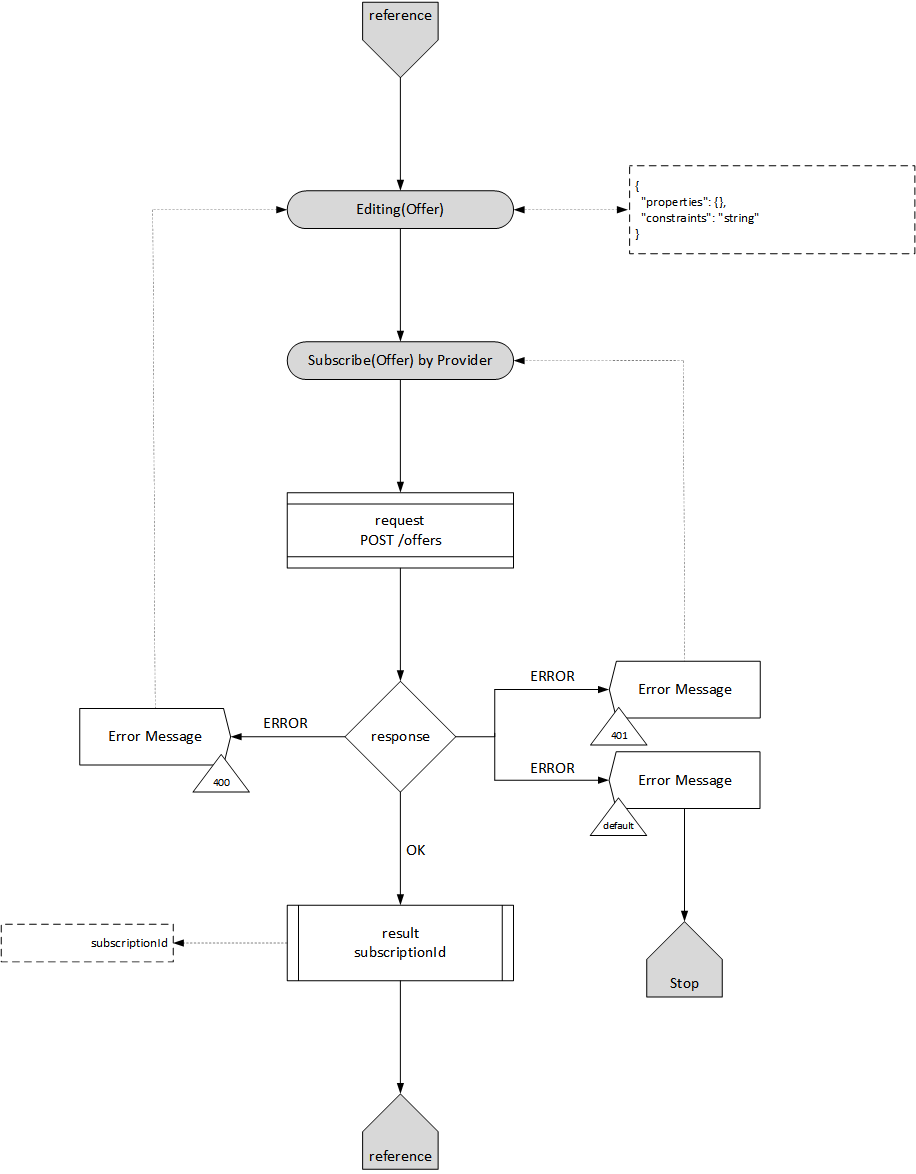
\includegraphics[width=12cm,height=12cm,angle=0]{./diag/Workflow/Market/SubscribeOffer-P-Workflow.png}
    \caption{Provider SubscribeOffer Workflow}
	\label{fig:SubsOffer}
\end{figure}

\end{enumerate}

\newpage

%% Unsubscribe Offer 
\subsubsubsection{UnsubscribeOffer Function}

\begin{enumerate}

\item Profile

\begin{enumerate}

\item Description

The UnsubscribeOffer function is used to stop receiving Demand Proposals for a Provider from Golem Market. 
It uses the DELETE /offers/\{subscriptionId\} method.

\item Side

Provider

\end{enumerate}

\item Request

\begin{enumerate}

\item Input

\begin{tcolorbox}[boxrule=0pt, frame empty]
\begin{verbatim}

subscriptionId

\end{verbatim}
\end{tcolorbox}

%Object

%\begin{tcolorbox}[boxrule=0pt, frame empty]
%\begin{verbatim}

%{
%  "properties": {},
%  "constraints": "string"
%}

%\end{verbatim}
%\end{tcolorbox}

\begin{table}[H]
\footnotesize

\begin{center}
\begin{tabular}{|p{3cm}|l|p{3cm}|p{3cm}|p{4cm}|} 
\hline
\rowcolor{lightgray}	Name	& MO.	& Type	& Example & 	Description \\
\hline

subscriptionId	& M	& 	string	&		&	Subscription Identifier \\ 

\hline

\end{tabular}
\end{center}

\end{table}

\item REST Method

\begin{tcolorbox}[boxrule=0pt, frame empty]
\begin{verbatim} 

DELETE /offers/{subscriptionId}

\end{verbatim}
\end{tcolorbox}

\end{enumerate}

\item Response

\begin{table}[H]
\footnotesize

\begin{center}
\begin{tabular}{|c|l|} 
\hline
\rowcolor{lightgray}	Code 		& 	Description \\
\hline
204	 		&	Offer revoked \\
\hline
%400			&	(400) Bad request \\
%\hline
401			&	(401) Authorization information is missing or invalid. \\
\hline
410			&	Already unsubscribed. \\
\hline
default		&	Unexpected error. \\
\hline
\end{tabular}
\end{center}

\end{table}

\item Result

\begin{tcolorbox}[boxrule=0pt, frame empty]
\begin{verbatim}

None

\end{verbatim}
\end{tcolorbox}

%\begin{center}
%\begin{tabular}{|p{3cm}|l|p{3cm}|p{3cm}|p{4cm}|} 
%\hline
%\rowcolor{lightgray}	Name	& MO.	& Type	& Example & 	Description \\
%\hline

%subscriptionId	&	& 	string	&		&	Subscription Identifier \\ 

%\hline

%\end{tabular}
%\end{center}


\item Workflow

(Please see Figure ~\ref{fig:UsO} on page ~\pageref{fig:UsO}):

\begin{figure}[H]
    \centering
    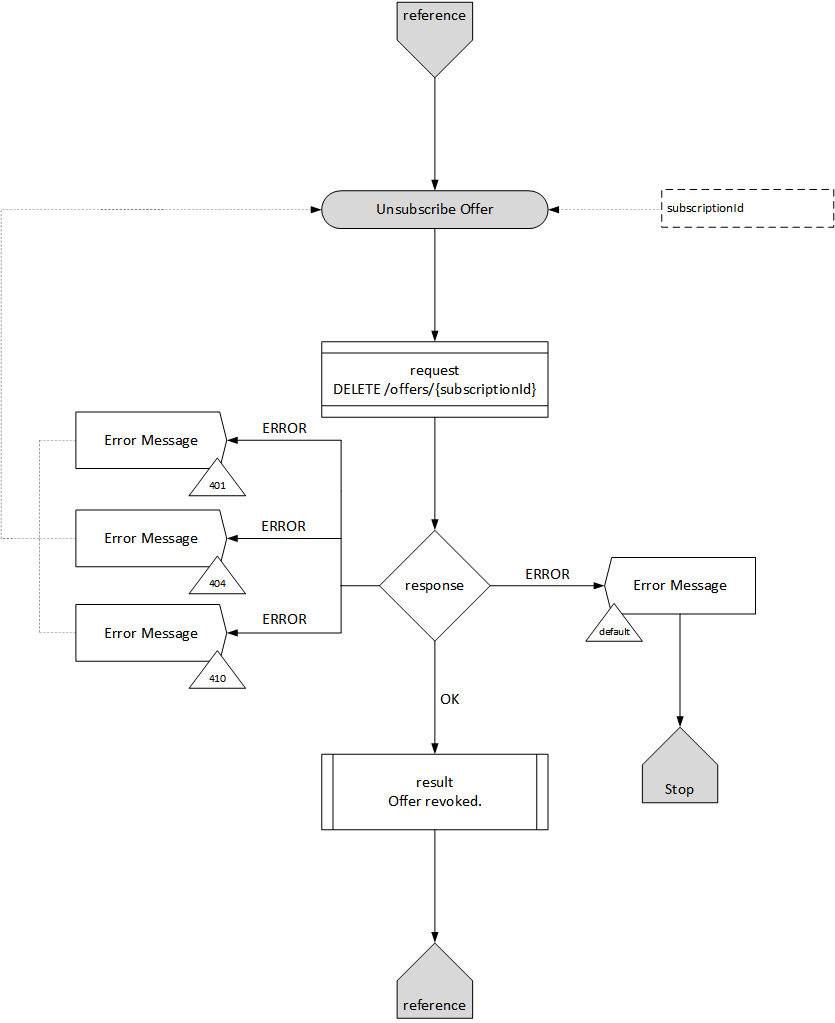
\includegraphics[width=12cm,height=12cm,angle=0]{./diag/Workflow/Market/UnsubscribeOffer-P-Workflow.png}
    \caption{Provider UnsubscribeOffer Workflow}
	\label{fig:UsO}
\end{figure}

\end{enumerate}

\newpage

\subsubsubsection{List(GetOffers) Function}

\begin{enumerate}

\item Profile

\begin{enumerate}

\item Description

The GetOffers function is used to fetch all active Offers which have been published by the Provider. 
It uses the GET /offers method.

\item Side

Provider

\end{enumerate}

\item Request

\begin{enumerate}

\item Input

\begin{tcolorbox}[boxrule=0pt, frame empty]
\begin{verbatim}

No parameters

\end{verbatim}
\end{tcolorbox}

%Offer Object

%\begin{tcolorbox}[boxrule=0pt, frame empty]
%\begin{verbatim}

%{
%  "properties": {},
%  "constraints": "string"
%}

%\end{verbatim}
%\end{tcolorbox}

%\begin{center}
%\begin{tabular}{|p{3cm}|l|p{3cm}|p{3cm}|p{4cm}|} 
%\hline
%\rowcolor{lightgray}	Name	& MO.	& Type	& Example & 	Description \\
%\hline

%properties	& M	& 	json or flat	&		&	Offer properties \\ 

%\hline

%constraints	& O	& 	string	&		&	Offer constraints \\ 

%\hline

%\end{tabular}
%\end{center}

\item REST Method

\begin{tcolorbox}[boxrule=0pt, frame empty]
\begin{verbatim} 

GET /offers

\end{verbatim}
\end{tcolorbox}

\end{enumerate}

\item Response

\begin{table}[H]
\footnotesize

\begin{center}
\begin{tabular}{|c|l|} 
\hline
\rowcolor{lightgray}	Code 		& 	Description \\
\hline
200	 		&	Offer list. \\
\hline
400			&	(400) Bad request \\
\hline
401			&	(401) Authorization information is missing or invalid. \\
\hline
default		&	Unexpected error. \\
\hline
\end{tabular}
\end{center}

\end{table}

\item Result

\begin{tcolorbox}[boxrule=0pt, frame empty]
\begin{verbatim}

[
  {
    "properties": {},
    "constraints": "string",
    "offerId": "string",
    "providerId": "string",
    "timestamp": "YYYY-MM-DDThh:mm:ss.sssZ"
  }
]

\end{verbatim}
\end{tcolorbox}

\begin{table}[H]
\footnotesize

\begin{center}
\begin{tabular}{|p{3cm}|l|p{3cm}|p{3cm}|p{4cm}|} 
\hline
\rowcolor{lightgray}	Name	& MO.	& Type	& Example & 	Description \\
\hline

properties	& 	& 	json or flat	&		&	Offer properties \\ 

\hline

constraints	& 	& 	string	&		&	Offer constraints \\ 

\hline

offerId		&	&	string	&		& 	Offer Identifier \\

\hline

providerId  & 	&	string	&		&	Provider's Node Identifier \\

\hline

timestamp	&	& 	string(\$date-time)	& YYYY-MM-DDThh:mm:ss.sssZ	&	Time of ???  \\ 

\hline

\end{tabular}
\end{center}

\end{table}

\item Workflow

(Please see Figure ~\ref{fig:LO} on page ~\pageref{fig:LO}):

\begin{figure}[H]
    \centering
    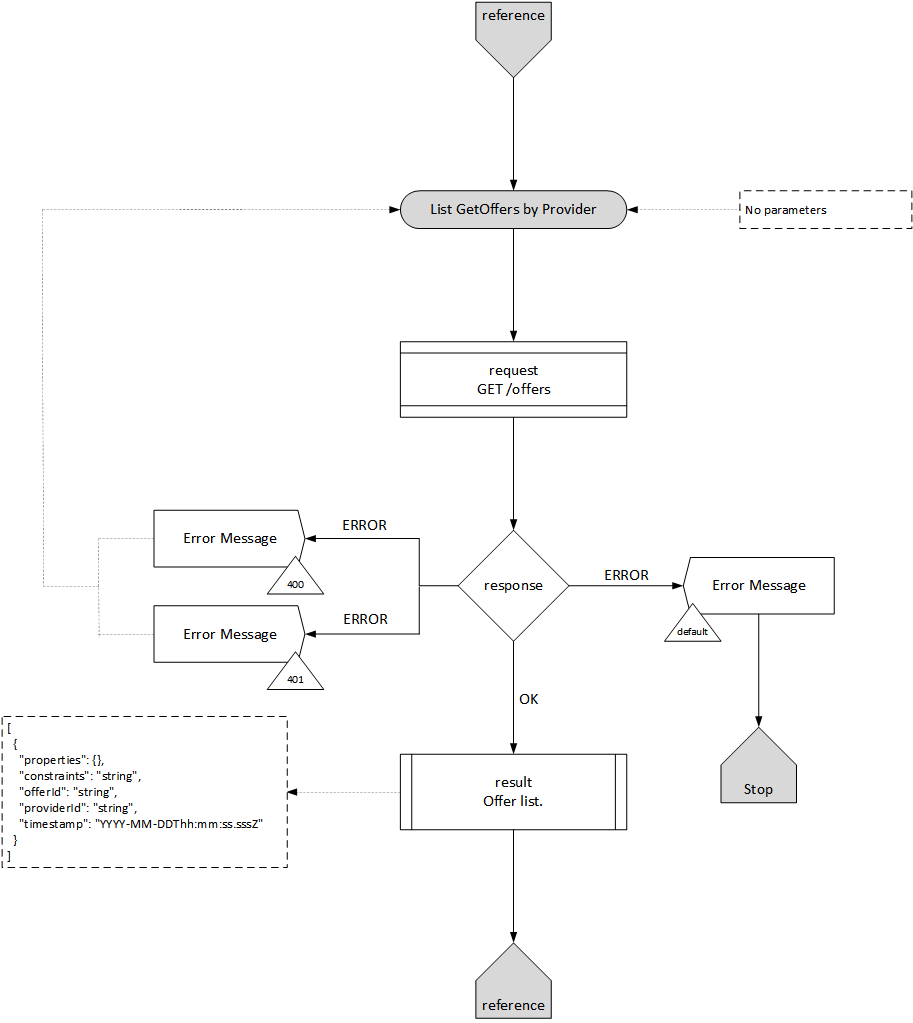
\includegraphics[width=12cm,height=12cm,angle=0]{./diag/Workflow/Market/List(GetOffers)-P-Workflow.png}
    \caption{Provider Workflow Active Offer List }
	\label{fig:LO}
\end{figure}


\end{enumerate}

\newpage

\subsubsubsection{CollectDemands Function}

\begin{enumerate}

\item Profile

\begin{enumerate}

\item Description

The CollectDemands function is used to read Market responses to published Offer by the Provider. 
It uses the GET /offers/\{subscriptionId\}/events method.

\item Side

Provider

\end{enumerate}

\item Request

\begin{enumerate}

\item Input

\begin{tcolorbox}[boxrule=0pt, frame empty]
\begin{verbatim}

subscriptionId
timeout
maxEvents

\end{verbatim}
\end{tcolorbox}

%Offer Object
%\begin{tcolorbox}[boxrule=0pt, frame empty]
%\begin{verbatim}
%{
%  "properties": {},
%  "constraints": "string"
%}
%\end{verbatim}
%\end{tcolorbox}

\begin{table}[H]
\footnotesize

\begin{center}
\begin{tabular}{|p{3cm}|l|p{3cm}|p{3cm}|p{4cm}|} 
\hline
\rowcolor{lightgray}	Name	& MO.	& Type	& Example & 	Description \\
\hline

subscriptionId	& M	& 	string			&		&	Subscription Identifier \\ 

\hline

timeout			& O	& 	number(\$float)	&		&	Timeout used in long-polling calls (in seconds). 
													How many seconds server should wait for response containing new events 
													(0.0 means it should return immediately if there are no events).	Default value : 5 \\ 

\hline

maxEvents		& O & integer(\$int32)	&		&	Maximum number of events that server should return at once.		Default value : 10 \\

\hline	

\end{tabular}
\end{center}

\end{table}

\item REST Method

\begin{tcolorbox}[boxrule=0pt, frame empty]
\begin{verbatim} 

GET /offers/{subscriptionId}/events

\end{verbatim}
\end{tcolorbox}

\end{enumerate}

\item Response

\begin{table}[H]
\footnotesize

\begin{center}
\begin{tabular}{|c|l|} 
\hline
\rowcolor{lightgray}	Code 		& 	Description \\
\hline
200	 		&	Proposal or Agreement event list. \\
\hline
404			&	(404) The specified resource was not found. \\
\hline
401			&	(401) Authorization information is missing or invalid. \\
\hline
default		&	Unexpected error. \\
\hline
\end{tabular}
\end{center}

\end{table}

\item Result

\begin{tcolorbox}[boxrule=0pt, frame empty]
\begin{verbatim}

[
  {
    "eventType": "string",
    "eventDate": "YYYY-MM-DDThh:mm:ss.sssZ"
  }
]

\end{verbatim}
\end{tcolorbox}

\begin{table}[H]
\footnotesize

\begin{center}
\begin{tabular}{|p{3cm}|l|p{3cm}|p{3cm}|p{4cm}|} 
\hline
\rowcolor{lightgray}	Name	& MO.	& Type	& Example & 	Description \\
\hline

eventType	& 	& 	string	&		&	Event Type \\ 

\hline

eventDate	& 	& 	string(\$date-time)	&	YYYY-MM-DDThh:mm:ss.sssZ	&	Event Date \\ 

\hline

\end{tabular}
\end{center}

\end{table}

\item Workflow

(Please see Figure ~\ref{fig:CD} on page ~\pageref{fig:CD}):

\begin{figure}[H]
    \centering
    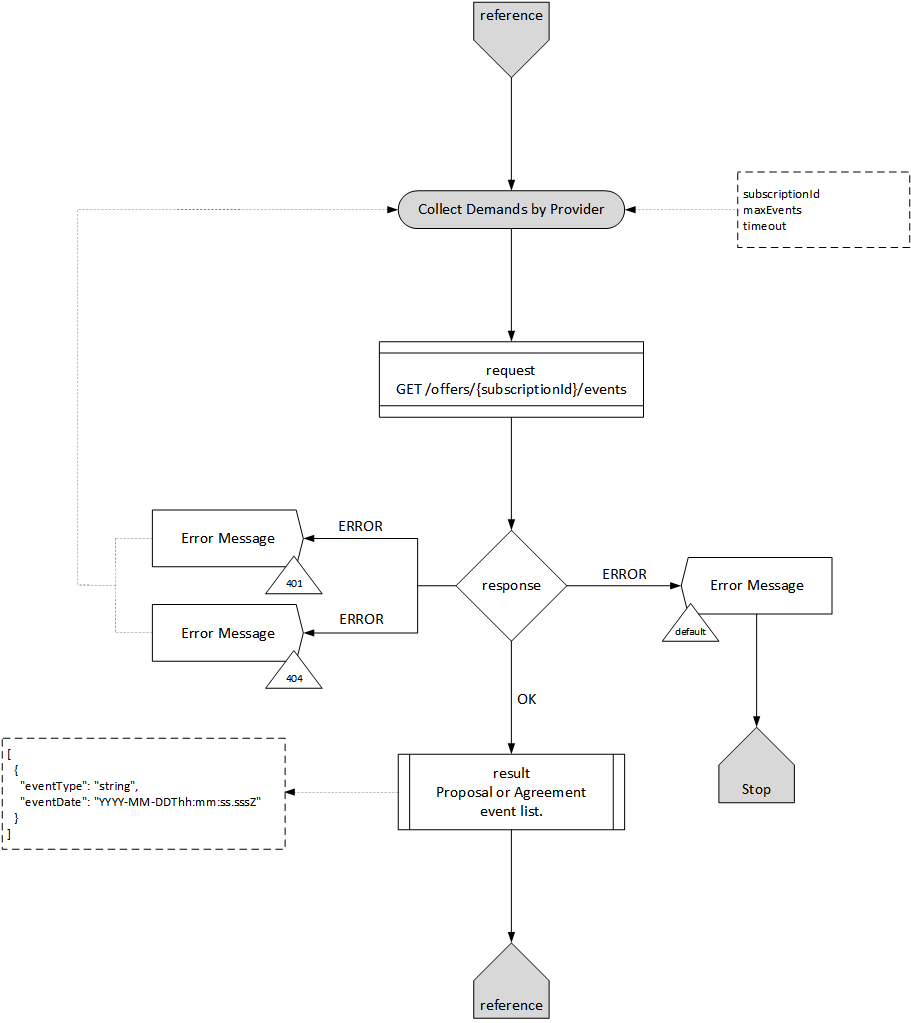
\includegraphics[width=11cm,height=11cm,angle=0]{./diag/Workflow/Market/CollectDemads-P-Workflow.png}
    \caption{Provider Workflow Collect Demands }
	\label{fig:CD}
\end{figure}

\end{enumerate}

\newpage

\subsubsubsection{GetProposalDemand Function}

\begin{enumerate}

\item Profile

\begin{enumerate}

\item Description

The GetProposalDemand function is used to fetch Proposal (Demand) with given id. 
It uses the GET /offers/\{subscriptionId\}/proposals/\{proposalId\} method.

\item Side

Provider

\end{enumerate}

\item Request

\begin{enumerate}

\item Input

\begin{tcolorbox}[boxrule=0pt, frame empty]
\begin{verbatim}

subscriptionId
proposalId

\end{verbatim}
\end{tcolorbox}

%Object
%\begin{tcolorbox}[boxrule=0pt, frame empty]
%\begin{verbatim}
%{
%  "properties": {},
%  "constraints": "string"
%}
%\end{verbatim}
%\end{tcolorbox}

\begin{table}[H]
\footnotesize

\begin{center}
\begin{tabular}{|p{3cm}|l|p{3cm}|p{3cm}|p{4cm}|} 
\hline
\rowcolor{lightgray}	Name	& MO.	& Type	& Example & 	Description \\
\hline

subscriptionId	& M	& 	string			&		&	Subscription Identifier \\ 

\hline

proposalId		& M & 	string			&		&	Proposal Identifier \\

\hline	

\end{tabular}
\end{center}

\end{table}

\item REST Method

\begin{tcolorbox}[boxrule=0pt, frame empty]
\begin{verbatim} 

GET /offers/{subscriptionId}/proposals/{proposalId}

\end{verbatim}
\end{tcolorbox}

\end{enumerate}

\item Response

\begin{table}[H]
\footnotesize

\begin{center}
\begin{tabular}{|c|l|} 
\hline
\rowcolor{lightgray}	Code 		& 	Description \\
\hline
200	 		&	Proposal  \\
\hline
404			&	(404) The specified resource was not found. \\
\hline
401			&	(401) Authorization information is missing or invalid. \\
\hline
410			&	Proposal rejected. \\
\hline
default		&	Unexpected error. \\
\hline
\end{tabular}
\end{center}

\end{table}

\item Result

\begin{tcolorbox}[boxrule=0pt, frame empty]
\begin{verbatim}

{
  "properties": {},
  "constraints": "string",
  "proposalId": "string",
  "issuerId": "string",
  "state": "Initial",
  "timestamp": "YYYY-MM-DDThh:mm:ss.sssZ",
  "prevProposalId": "string"
}

\end{verbatim}
\end{tcolorbox}

\begin{table}[H]
\footnotesize

\begin{center}
\begin{tabular}{|p{3cm}|l|p{3cm}|p{3cm}|p{4cm}|} 
\hline
\rowcolor{lightgray}	Name	& MO.	& Type	& Example & 	Description \\
\hline

properties	& 	& 	json or flat		&								&	 \\ 

\hline

constraints &	&	string				&								&	\\

\hline

proposalId	&	&	string				&								& Proposal Identifier \\

\hline

issuerId	&	&	string				&								& Issuer Node Id \\

\hline

state		&	&	enum				& [Initial, Draft, Rejected, Accepted, Expired] & Proposal State \\

\hline

timestamp	& 	& 	string(\$date-time)	&	YYYY-MM-DDThh:mm:ss.sssZ	&	Time ? \\ 

\hline

prevProposalId & &	string 				&								&	Id of the proposal from other side which this proposal responds to \\

\hline

\end{tabular}
\end{center}

\end{table}

\item Workflow

(Please see Figure ~\ref{fig:GPD} on page ~\pageref{fig:GPD}):

\begin{figure}[H]
    \centering
    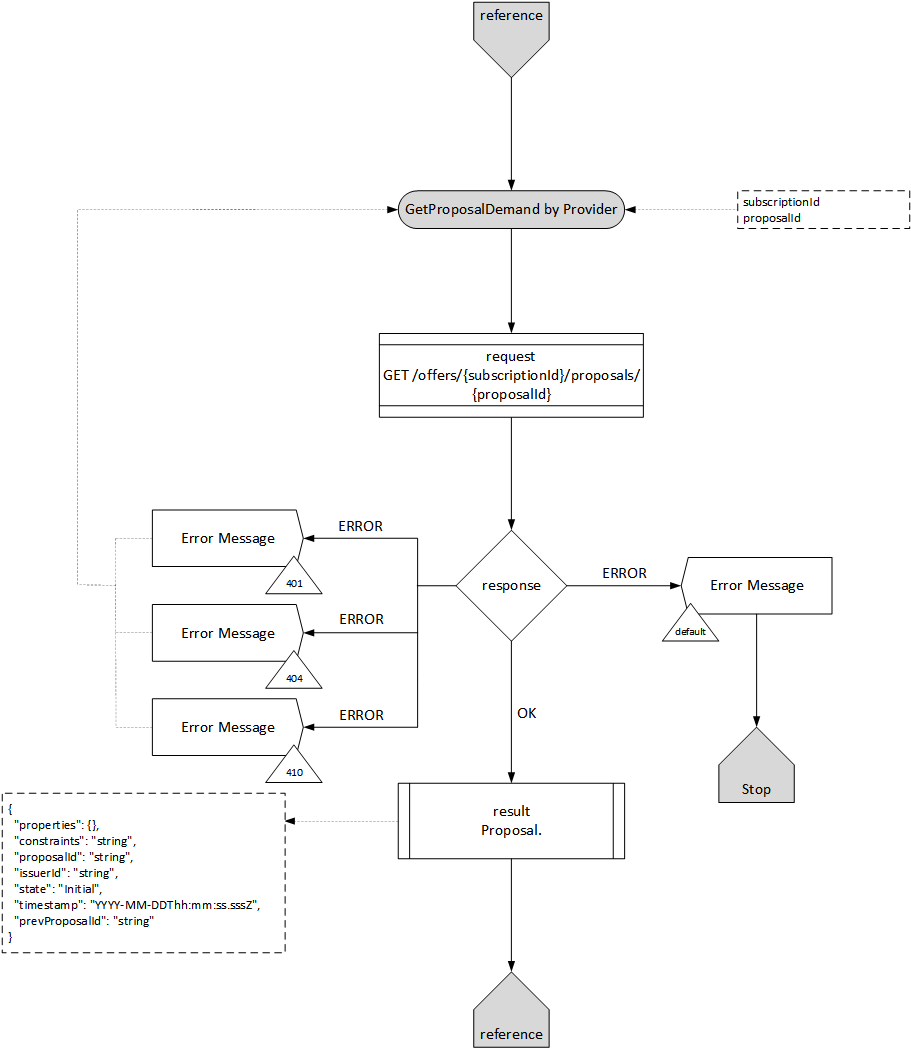
\includegraphics[width=12cm,height=12cm,angle=0]{./diag/Workflow/Market/GetProposalDemand-P-Workflow.png}
    \caption{Provider Workflow Get Proposal Demand }
	\label{fig:GPD}
\end{figure}

\end{enumerate}

\newpage

\subsubsubsection{CounterProposalOffer Function}

\begin{enumerate}

\item Profile

\begin{enumerate}

\item Description

The CounterProposalOffer function is used to respond with bespoke Offer to received Demand. 
It uses the POST /offers/\{subscriptionId\}/proposals/\{proposalId\} method.

\item Side

Provider

\end{enumerate}

\item Request

\begin{enumerate}

\item Input

\begin{tcolorbox}[boxrule=0pt, frame empty]
\begin{verbatim}

subscriptionId
proposalId

\end{verbatim}
\end{tcolorbox}

Offer Object
\begin{tcolorbox}[boxrule=0pt, frame empty]
\begin{verbatim}
{
  "properties": {},
  "constraints": "string"
}
\end{verbatim}
\end{tcolorbox}

\begin{table}[H]
\footnotesize

\begin{center}
\begin{tabular}{|p{3cm}|l|p{3cm}|p{3cm}|p{4cm}|} 
\hline
\rowcolor{lightgray}	Name	& MO.	& Type	& Example & 	Description \\
\hline

subscriptionId	& M	& 	string			&		&	Subscription Identifier \\ 
\hline

proposalId		& M & 	string			&		&	Proposal Identifier \\
\hline	

properties		& M &	json or flat 	&		& Offer Properties		\\
\hline

constraints 	& M &	string			&		& Offer Constraints		\\
\hline

\end{tabular}
\end{center}

\end{table}

\item REST Method

\begin{tcolorbox}[boxrule=0pt, frame empty]
\begin{verbatim} 

POST /offers/{subscriptionId}/proposals/{proposalId}

\end{verbatim}
\end{tcolorbox}

\end{enumerate}

\item Response

\begin{table}[H]
\footnotesize

\begin{center}
\begin{tabular}{|c|l|} 
\hline
\rowcolor{lightgray}	Code 		& 	Description \\
\hline
201	 		&	Counter Proposal created.  \\
\hline
400			&	(400) Bad request	\\
\hline
404			&	(404) The specified resource was not found. \\
\hline
401			&	(401) Authorization information is missing or invalid. \\
\hline
410			&	Proposal rejected. \\
\hline
default		&	Unexpected error. \\
\hline
\end{tabular}
\end{center}

\end{table}

\item Result

\begin{tcolorbox}[boxrule=0pt, frame empty]
\begin{verbatim}
  proposalId
\end{verbatim}
\end{tcolorbox}

\begin{table}[H]
\footnotesize

\begin{center}
\begin{tabular}{|p{3cm}|l|p{3cm}|p{3cm}|p{4cm}|} 
\hline
\rowcolor{lightgray}	Name	& MO.	& Type	& Example & 	Description \\
\hline

proposalId	&	&	string				&								& Proposal Identifier \\
\hline

\end{tabular}
\end{center}

\end{table}

\item Workflow

(Please see Figure ~\ref{fig:CPO} on page ~\pageref{fig:CPO}):

\begin{figure}[H]
    \centering
    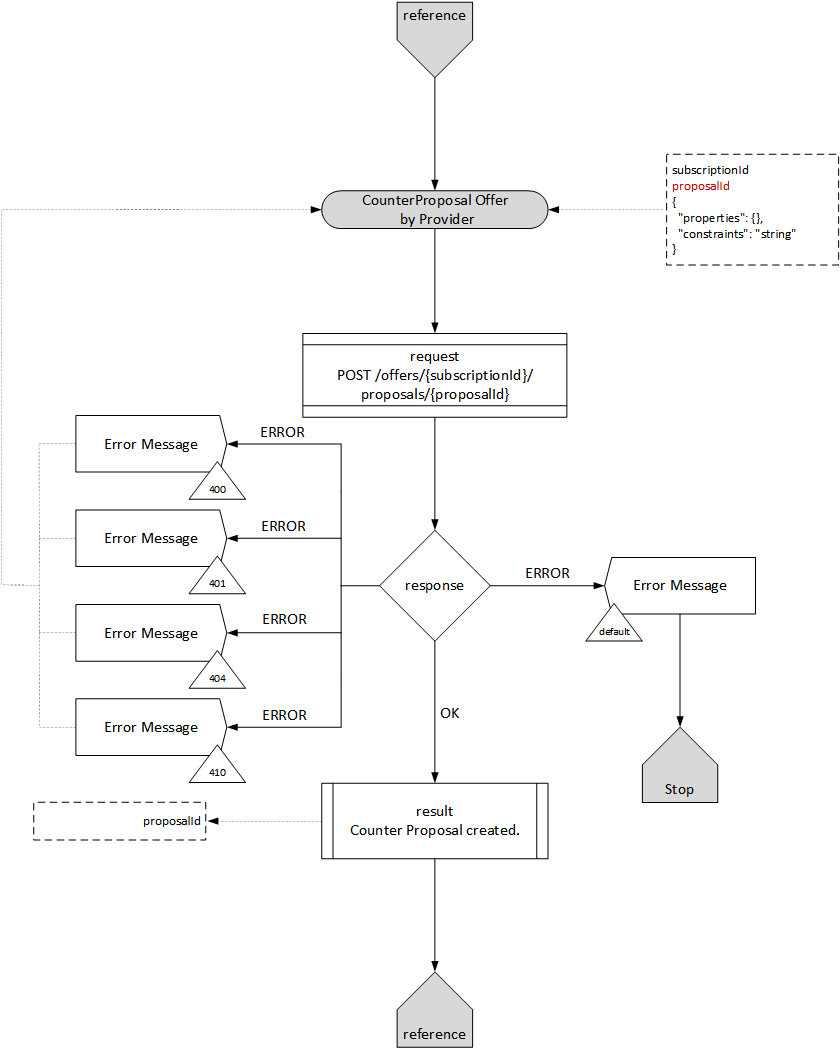
\includegraphics[width=12cm,height=12cm,angle=0]{./diag/Workflow/Market/CounterProposalOffer-P-Workflow.png}
    \caption{Provider Workflow Counter Proposal Offer }
	\label{fig:CPO}
\end{figure}

\end{enumerate}

\newpage

\subsubsubsection{RejectProposalDemand Function}

\begin{enumerate}

\item Profile

\begin{enumerate}

\item Description

The RejectProposalDemand function is used to reject Proposal Demand. \\
It uses the POST /offers/\{subscriptionId\}/proposals/\{proposalId\}/reject method.

\item Side

Provider

\end{enumerate}

\item Request

\begin{enumerate}

\item Input

\begin{tcolorbox}[boxrule=0pt, frame empty]
\begin{verbatim}

subscriptionId
proposalId

\end{verbatim}
\end{tcolorbox}

Object
\begin{tcolorbox}[boxrule=0pt, frame empty]
\begin{verbatim}
{
  "message": "string",
  "additionalProp1": {}
}
\end{verbatim}
\end{tcolorbox}

\begin{table}[H]
\footnotesize

\begin{center}
\begin{tabular}{|p{3cm}|l|p{3cm}|p{3cm}|p{4cm}|} 
\hline
\rowcolor{lightgray}	Name	& MO.	& Type	& Example & 	Description \\
\hline

subscriptionId		& M	& 	string			&		&	Subscription Identifier \\ 
\hline

proposalId			& M & 	string			&		&	Proposal Identifier \\
\hline	

message				& O &	string 			&		& 		\\
\hline

additionalProp1 	& O &	json			&		& 		\\
\hline

\end{tabular}
\end{center}

\end{table}

\item REST Method

\begin{tcolorbox}[boxrule=0pt, frame empty]
\begin{verbatim} 

POST /offers/{subscriptionId}/proposals/{proposalId}/reject

\end{verbatim}
\end{tcolorbox}

\end{enumerate}

\item Response

\begin{table}[H]
\footnotesize

\begin{center}
\begin{tabular}{|c|l|} 
\hline
\rowcolor{lightgray}	Code 		& 	Description \\
\hline
204	 		&	Proposal rejected.  \\
\hline
404			&	(404) The specified resource was not found. \\
\hline
401			&	(401) Authorization information is missing or invalid. \\
\hline
410			&	Proposal rejected. \\
\hline
default		&	Unexpected error. \\
\hline
\end{tabular}
\end{center}

\end{table}

\item Result

\begin{tcolorbox}[boxrule=0pt, frame empty]
\begin{verbatim}
  None
\end{verbatim}
\end{tcolorbox}

\item Workflow

(Please see Figure ~\ref{fig:RPD} on page ~\pageref{fig:RPD}):

\begin{figure}[H]
    \centering
    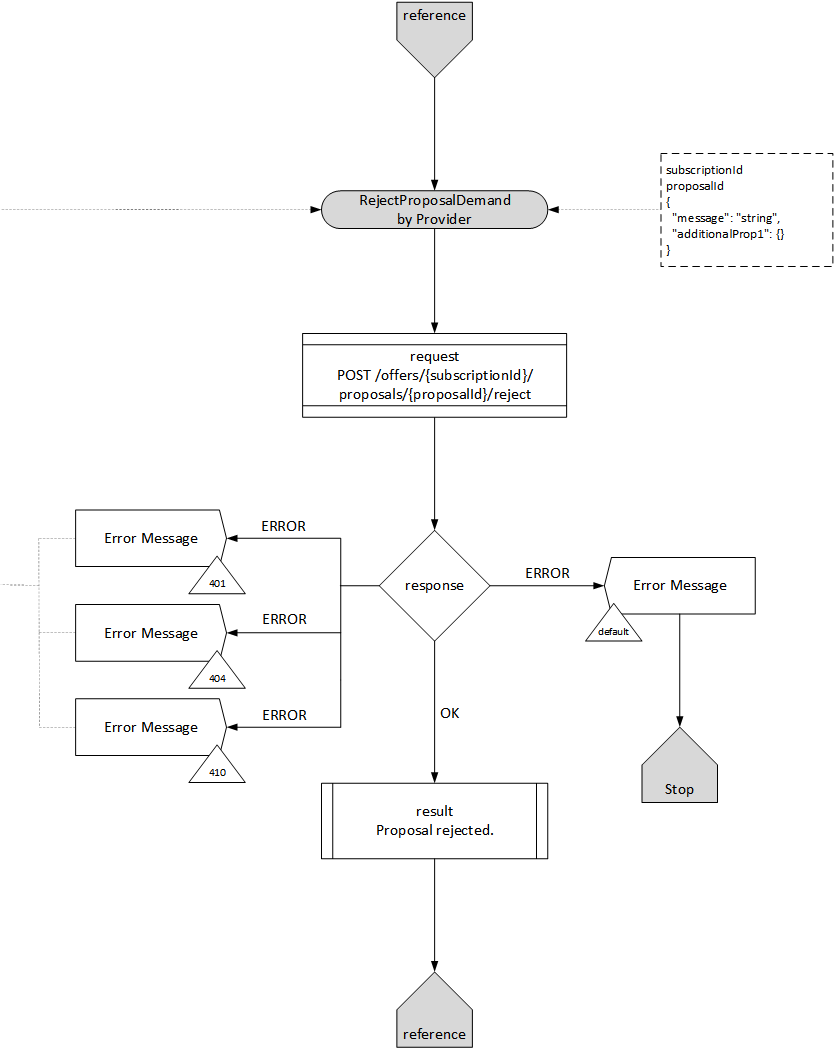
\includegraphics[width=12cm,height=12cm,angle=0]{./diag/Workflow/Market/RejectProposalDemand-P-Workflow.png}
    \caption{Provider Workflow Reject Proposal Demand }
	\label{fig:RPD}
\end{figure}

\end{enumerate}

\newpage

%%%%%%%%% Demand %%%%%%%%%%%%%%%%%%%%%%%%%%%%%

\subsubsubsection{SubscribeDemand Function}

\begin{enumerate}

\item Profile

\begin{enumerate}

\item Description

The SubscribeDemand function is used to publish the Requestor Demand on the Golem Market. It uses the POST /demands method.
The Demand object is a set of properties and constraints of the item being ordered (e.g., computing resources such as CPU, MEM, HDD, GPU, NIC)

\item Side

Requestor

\end{enumerate}

\item Request

\begin{enumerate}

\item Input

\begin{tcolorbox}[boxrule=0pt, frame empty]
\begin{verbatim}

No parameters

\end{verbatim}
\end{tcolorbox}

Demand Object

\begin{tcolorbox}[boxrule=0pt, frame empty]
\begin{verbatim}

{
  "properties": {},
  "constraints": "string"
}

\end{verbatim}
\end{tcolorbox}

\begin{table}[H]
\footnotesize

\begin{center}
\begin{tabular}{|p{3cm}|l|p{3cm}|p{3cm}|p{4cm}|} 
\hline
\rowcolor{lightgray}	Name	& MO.	& Type	& Example & 	Description \\
\hline

properties	& M	& 	json or flat	&		&	Offer properties \\ 

\hline

constraints	& O	& 	string	&		&	Offer constraints \\ 

\hline

\end{tabular}
\end{center}

\end{table}

\item REST Method

\begin{tcolorbox}[boxrule=0pt, frame empty]
\begin{verbatim} 

POST /demands

\end{verbatim}
\end{tcolorbox}

\end{enumerate}

\item Response

\begin{table}[H]
\footnotesize

\begin{center}
\begin{tabular}{|c|l|} 
\hline
\rowcolor{lightgray}	Code 		& 	Description \\
\hline
201	 		&	Subscribed \\
\hline
400			&	(400) Bad request \\
\hline
401			&	(401) Authorization information is missing or invalid. \\
\hline
default		&	Unexpected error. \\
\hline
\end{tabular}
\end{center}

\end{table}

\item Result

\begin{tcolorbox}[boxrule=0pt, frame empty]
\begin{verbatim}

subscriptionId

\end{verbatim}
\end{tcolorbox}

\begin{table}[H]
\footnotesize

\begin{center}
\begin{tabular}{|p{3cm}|l|p{3cm}|p{3cm}|p{4cm}|} 
\hline
\rowcolor{lightgray}	Name	& MO.	& Type	& Example & 	Description \\
\hline

subscriptionId	&	& 	string	&		&	Subscription Identifier \\ 

\hline

\end{tabular}
\end{center}

\end{table}

\item Workflow

(Please see Figure ~\ref{fig:SubsDemand} on page ~\pageref{fig:SubsDemand}):

\begin{figure}[H]
    \centering
    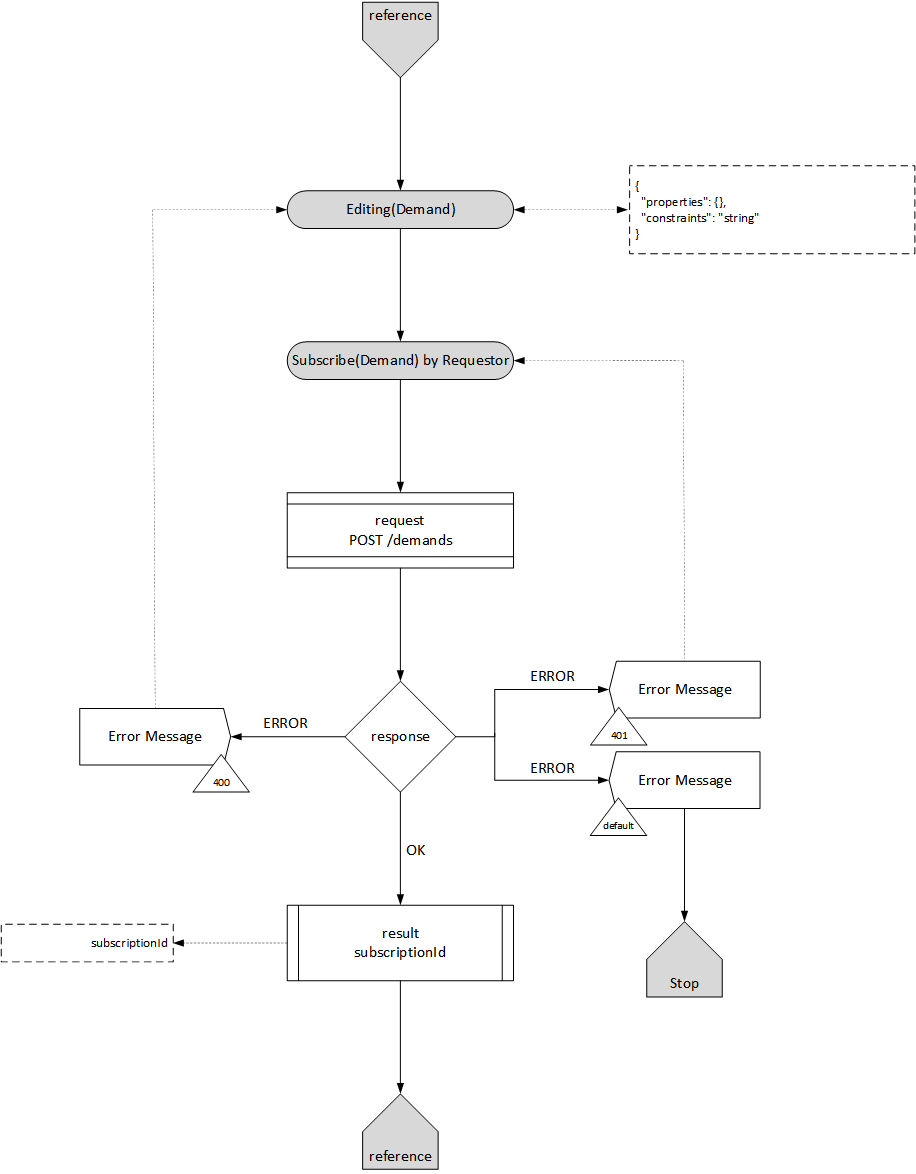
\includegraphics[width=12cm,height=12cm,angle=0]{./diag/Workflow/Market/SubscribeDemand-R-Workflow.png}
    \caption{Requestor SubscribeDemand Workflow}
	\label{fig:SubsDemand}
\end{figure}

\end{enumerate}

\newpage

%% Unsubscribe Demand 
\subsubsubsection{UnsubscribeDemand Function}

\begin{enumerate}

\item Profile

\begin{enumerate}

\item Description

The UnsubscribeDemand function is used to stop receiving Offer Proposals for a Requestor from Golem Market. \\ 
It uses the DELETE /demands/\{subscriptionId\} method.

\item Side

Requestor

\end{enumerate}

\item Request

\begin{enumerate}

\item Input

\begin{tcolorbox}[boxrule=0pt, frame empty]
\begin{verbatim}

subscriptionId

\end{verbatim}
\end{tcolorbox}

%Demand Object

%\begin{tcolorbox}[boxrule=0pt, frame empty]
%\begin{verbatim}

%{
%  "properties": {},
%  "constraints": "string"
%}

%\end{verbatim}
%\end{tcolorbox}

\begin{table}[H]
\footnotesize

\begin{center}
\begin{tabular}{|p{3cm}|l|p{3cm}|p{3cm}|p{4cm}|} 
\hline
\rowcolor{lightgray}	Name	& MO.	& Type	& Example & 	Description \\
\hline

subscriptionId	& M	& 	string	&		&	Subscription Identifier \\ 

\hline

\end{tabular}
\end{center}

\end{table}

\item REST Method

\begin{tcolorbox}[boxrule=0pt, frame empty]
\begin{verbatim} 

DELETE /demands/{subscriptionId}

\end{verbatim}
\end{tcolorbox}

\end{enumerate}

\item Response

\begin{table}[H]
\footnotesize

\begin{center}
\begin{tabular}{|c|l|} 
\hline
\rowcolor{lightgray}	Code 		& 	Description \\
\hline
204	 		&	Demand revoked \\
\hline
%400			&	(400) Bad request \\
%\hline
401			&	(401) Authorization information is missing or invalid. \\
\hline
410			&	Already unsubscribed. \\
\hline
default		&	Unexpected error. \\
\hline
\end{tabular}
\end{center}

\end{table}

\item Result

\begin{tcolorbox}[boxrule=0pt, frame empty]
\begin{verbatim}

None

\end{verbatim}
\end{tcolorbox}

%\begin{center}
%\begin{tabular}{|p{3cm}|l|p{3cm}|p{3cm}|p{4cm}|} 
%\hline
%\rowcolor{lightgray}	Name	& MO.	& Type	& Example & 	Description \\
%\hline

%subscriptionId	&	& 	string	&		&	Subscription Identifier \\ 

%\hline

%\end{tabular}
%\end{center}


\item Workflow

(Please see Figure ~\ref{fig:UsD} on page ~\pageref{fig:UsD}):

\begin{figure}[H]
    \centering
    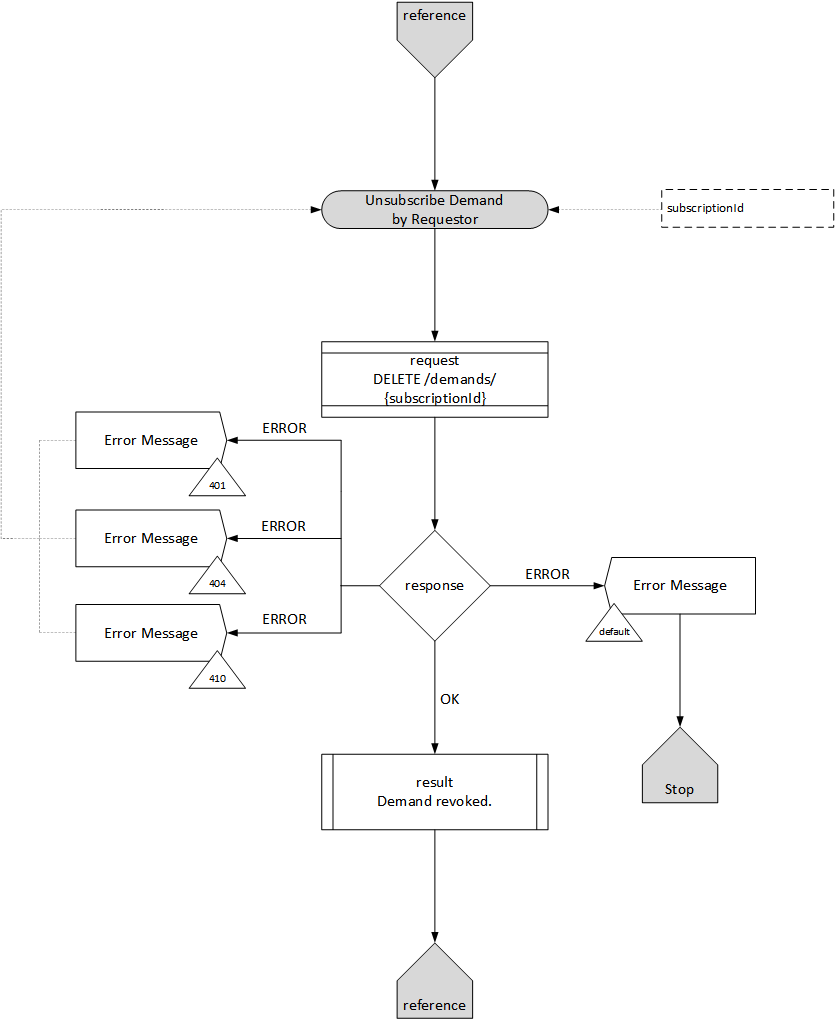
\includegraphics[width=12cm,height=12cm,angle=0]{./diag/Workflow/Market/UnsubsribeDemand-R-Workflow.png}
    \caption{Requestor UnsubscribeDemand Workflow}
	\label{fig:UsD}
\end{figure}

\end{enumerate}

\newpage

\subsubsubsection{List(GetDemands) Function}

\begin{enumerate}

\item Profile

\begin{enumerate}

\item Description

The GetDemands function is used to fetch all active Demands which have been published by the Requestor. \\ 
It uses the GET /offers method.

\item Side

Requestor

\end{enumerate}

\item Request

\begin{enumerate}

\item Input

\begin{tcolorbox}[boxrule=0pt, frame empty]
\begin{verbatim}

No parameters

\end{verbatim}
\end{tcolorbox}

\item REST Method

\begin{tcolorbox}[boxrule=0pt, frame empty]
\begin{verbatim} 

GET /offers

\end{verbatim}
\end{tcolorbox}

\end{enumerate}

\item Response

\begin{table}[H]
\footnotesize

\begin{center}
\begin{tabular}{|c|l|} 
\hline
\rowcolor{lightgray}	Code 		& 	Description \\
\hline
200	 		&	Demand list. \\
\hline
400			&	(400) Bad request \\
\hline
401			&	(401) Authorization information is missing or invalid. \\
\hline
default		&	Unexpected error. \\
\hline
\end{tabular}
\end{center}

\end{table}

\item Result

\begin{tcolorbox}[boxrule=0pt, frame empty]
\begin{verbatim}

[
  {
    "properties": {},
    "constraints": "string",
    "demandId": "string",
    "requestorId": "string",
    "timestamp": "YYYY-MM-DDThh:mm:ss.sssZ"
  }
]

\end{verbatim}
\end{tcolorbox}

\begin{table}[H]
\footnotesize

\begin{center}
\begin{tabular}{|p{3cm}|l|p{3cm}|p{3cm}|p{4cm}|} 
\hline
\rowcolor{lightgray}	Name	& MO.	& Type	& Example & 	Description \\
\hline

properties	& 	& 	json or flat	&		&	Demand properties \\ 
\hline

constraints	& 	& 	string	&		&	Demand constraints \\ 
\hline

demandId		&	&	string	&		& 	Demand Identifier \\
\hline

requestorId  & 	&	string	&		&	Requestor's Node Identifier \\
\hline

timestamp	&	& 	string(\$date-time)	& YYYY-MM-DDThh:mm:ss.sssZ	&	Time of ???  \\ 
\hline

\end{tabular}
\end{center}

\end{table}

\item Workflow

(Please see Figure ~\ref{fig:LD} on page ~\pageref{fig:LD}):

\begin{figure}[H]
    \centering
    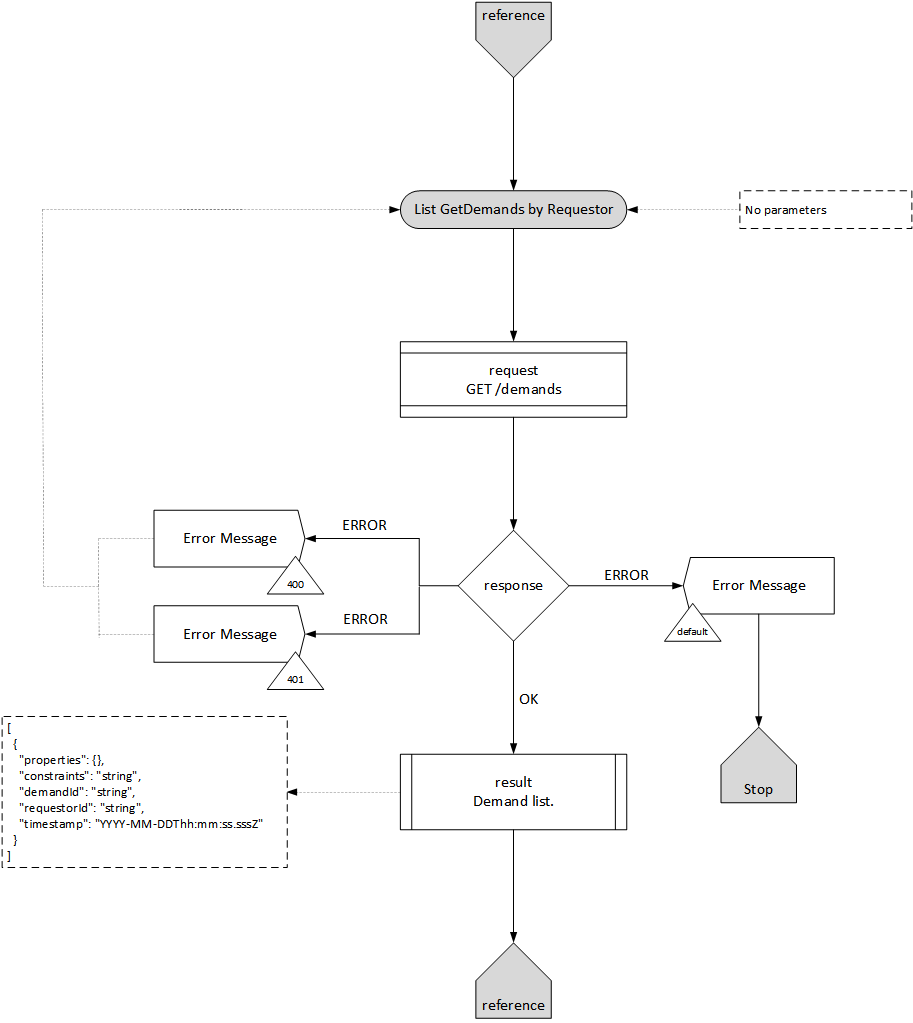
\includegraphics[width=12cm,height=12cm,angle=0]{./diag/Workflow/Market/List(GetDemands)-R-Workflow.png}
    \caption{Requestor Workflow Active Demand List }
	\label{fig:LD}
\end{figure}

\end{enumerate}

\newpage

\subsubsubsection{CollectOffers Function}

\begin{enumerate}

\item Profile

\begin{enumerate}

\item Description

The CollectOffers function is used to read Market responses to published Demand by the Requestor.  \\
It uses the GET /demands/\{subscriptionId\}/events method.

\item Side

Requestor

\end{enumerate}

\item Request

\begin{enumerate}

\item Input

\begin{tcolorbox}[boxrule=0pt, frame empty]
\begin{verbatim}

subscriptionId
timeout
maxEvents

\end{verbatim}
\end{tcolorbox}

%Offer Object
%\begin{tcolorbox}[boxrule=0pt, frame empty]
%\begin{verbatim}
%{
%  "properties": {},
%  "constraints": "string"
%}
%\end{verbatim}
%\end{tcolorbox}

\begin{table}[H]
\footnotesize

\begin{center}
\begin{tabular}{|p{3cm}|l|p{3cm}|p{3cm}|p{4cm}|} 
\hline
\rowcolor{lightgray}	Name	& MO.	& Type	& Example & 	Description \\
\hline

subscriptionId	& M	& 	string			&		&	Subscription Identifier \\ 

\hline

timeout			& O	& 	number(\$float)	&		&	Timeout used in long-polling calls (in seconds). 
													How many seconds server should wait for response containing new events 
													(0.0 means it should return immediately if there are no events).	Default value : 5 \\ 

\hline

maxEvents		& O & integer(\$int32)	&		&	Maximum number of events that server should return at once.		Default value : 10 \\

\hline	

\end{tabular}
\end{center}

\end{table}

\item REST Method

\begin{tcolorbox}[boxrule=0pt, frame empty]
\begin{verbatim} 

GET /demands/{subscriptionId}/events

\end{verbatim}
\end{tcolorbox}

\end{enumerate}

\item Response

\begin{table}[H]
\footnotesize

\begin{center}
\begin{tabular}{|c|l|} 
\hline
\rowcolor{lightgray}	Code 		& 	Description \\
\hline
200	 		&	Proposal or Agreement event list. \\
\hline
404			&	(404) The specified resource was not found. \\
\hline
401			&	(401) Authorization information is missing or invalid. \\
\hline
default		&	Unexpected error. \\
\hline
\end{tabular}
\end{center}

\end{table}

\item Result

\begin{tcolorbox}[boxrule=0pt, frame empty]
\begin{verbatim}

[
  {
    "eventType": "string",
    "eventDate": "YYYY-MM-DDThh:mm:ss.sssZ"
  }
]

\end{verbatim}
\end{tcolorbox}

\begin{table}[H]
\footnotesize

\begin{center}
\begin{tabular}{|p{3cm}|l|p{3cm}|p{3cm}|p{4cm}|} 
\hline
\rowcolor{lightgray}	Name	& MO.	& Type	& Example & 	Description \\
\hline

eventType	& 	& 	string	&		&	Event Type \\ 
\hline

eventDate	& 	& 	string(\$date-time)	&	YYYY-MM-DDThh:mm:ss.sssZ	&	Event Date \\ 
\hline

\end{tabular}
\end{center}

\end{table}

\item Workflow

(Please see Figure ~\ref{fig:CO} on page ~\pageref{fig:CO}):

\begin{figure}[H]
    \centering
    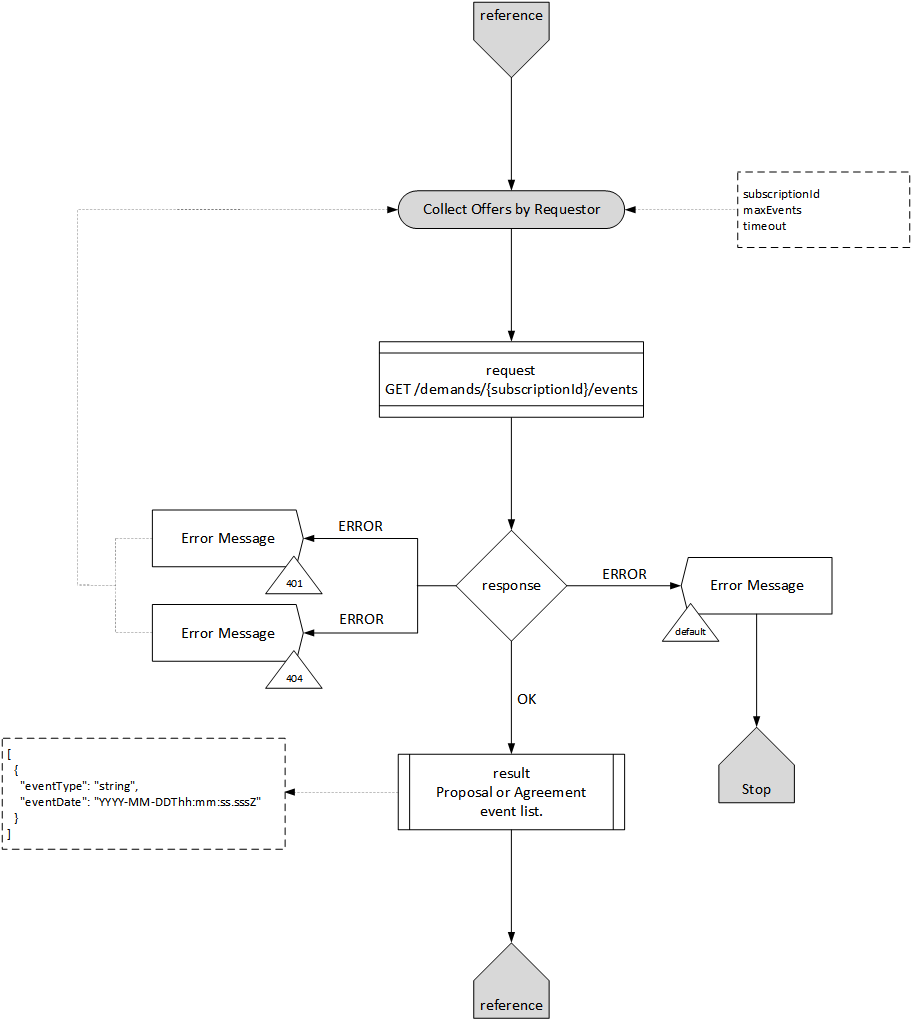
\includegraphics[width=11cm,height=11cm,angle=0]{./diag/Workflow/Market/CollectOffers-R-Workflow.png}
    \caption{Requestor Workflow Collect Offers }
	\label{fig:CO}
\end{figure}


\end{enumerate}

\newpage

\subsubsubsection{GetProposalOffer Function}

\begin{enumerate}

\item Profile

\begin{enumerate}

\item Description

The GetProposalOffer function is used to fetch Proposal (Offer) with given id. \\
It uses the GET /demands/\{subscriptionId\}/proposals/\{proposalId\} method.

\item Side

Requestor

\end{enumerate}

\item Request

\begin{enumerate}

\item Input

\begin{tcolorbox}[boxrule=0pt, frame empty]
\begin{verbatim}

subscriptionId
proposalId

\end{verbatim}
\end{tcolorbox}

%Offer Object
%\begin{tcolorbox}[boxrule=0pt, frame empty]
%\begin{verbatim}
%{
%  "properties": {},
%  "constraints": "string"
%}
%\end{verbatim}
%\end{tcolorbox}

\begin{table}[H]
\footnotesize

\begin{center}
\begin{tabular}{|p{3cm}|l|p{3cm}|p{3cm}|p{4cm}|} 
\hline
\rowcolor{lightgray}	Name	& MO.	& Type	& Example & 	Description \\
\hline

subscriptionId	& M	& 	string			&		&	Subscription Identifier \\ 
\hline

proposalId		& M & 	string			&		&	Proposal Identifier \\
\hline	

\end{tabular}
\end{center}

\end{table}

\item REST Method

\begin{tcolorbox}[boxrule=0pt, frame empty]
\begin{verbatim} 

GET /demands/{subscriptionId}/proposals/{proposalId}

\end{verbatim}
\end{tcolorbox}

\end{enumerate}

\item Response

\begin{table}[H]
\footnotesize

\begin{center}
\begin{tabular}{|c|l|} 
\hline
\rowcolor{lightgray}	Code 		& 	Description \\
\hline
200	 		&	Proposal  \\
\hline
404			&	(404) The specified resource was not found. \\
\hline
401			&	(401) Authorization information is missing or invalid. \\
\hline
410			&	Proposal rejected. \\
\hline
default		&	Unexpected error. \\
\hline
\end{tabular}
\end{center}

\end{table}

\item Result

\begin{tcolorbox}[boxrule=0pt, frame empty]
\begin{verbatim}

{
  "properties": {},
  "constraints": "string",
  "proposalId": "string",
  "issuerId": "string",
  "state": "Initial",
  "timestamp": "YYYY-MM-DDThh:mm:ss.sssZ",
  "prevProposalId": "string"
}

\end{verbatim}
\end{tcolorbox}

\begin{table}[H]
\footnotesize

\begin{center}
\begin{tabular}{|p{3cm}|l|p{3cm}|p{3cm}|p{4cm}|} 
\hline
\rowcolor{lightgray}	Name	& MO.	& Type	& Example & 	Description \\
\hline

properties	& 	& 	json or flat		&								&	 \\ 
\hline

constraints &	&	string				&								&	\\
\hline

proposalId	&	&	string				&								& Proposal Identifier \\
\hline

issuerId	&	&	string				&								& Issuer Node Id \\
\hline

state		&	&	enum				& [Initial, Draft, Rejected, Accepted, Expired] & Proposal State \\
\hline

timestamp	& 	& 	string(\$date-time)	&	YYYY-MM-DDThh:mm:ss.sssZ	&	Time ? \\ 
\hline

prevProposalId & &	string 				&								&	Id of the proposal from other side which this proposal responds to \\
\hline

\end{tabular}
\end{center}

\end{table}

\item Workflow

(Please see Figure ~\ref{fig:GPO} on page ~\pageref{fig:GPO}):

\begin{figure}[H]
    \centering
    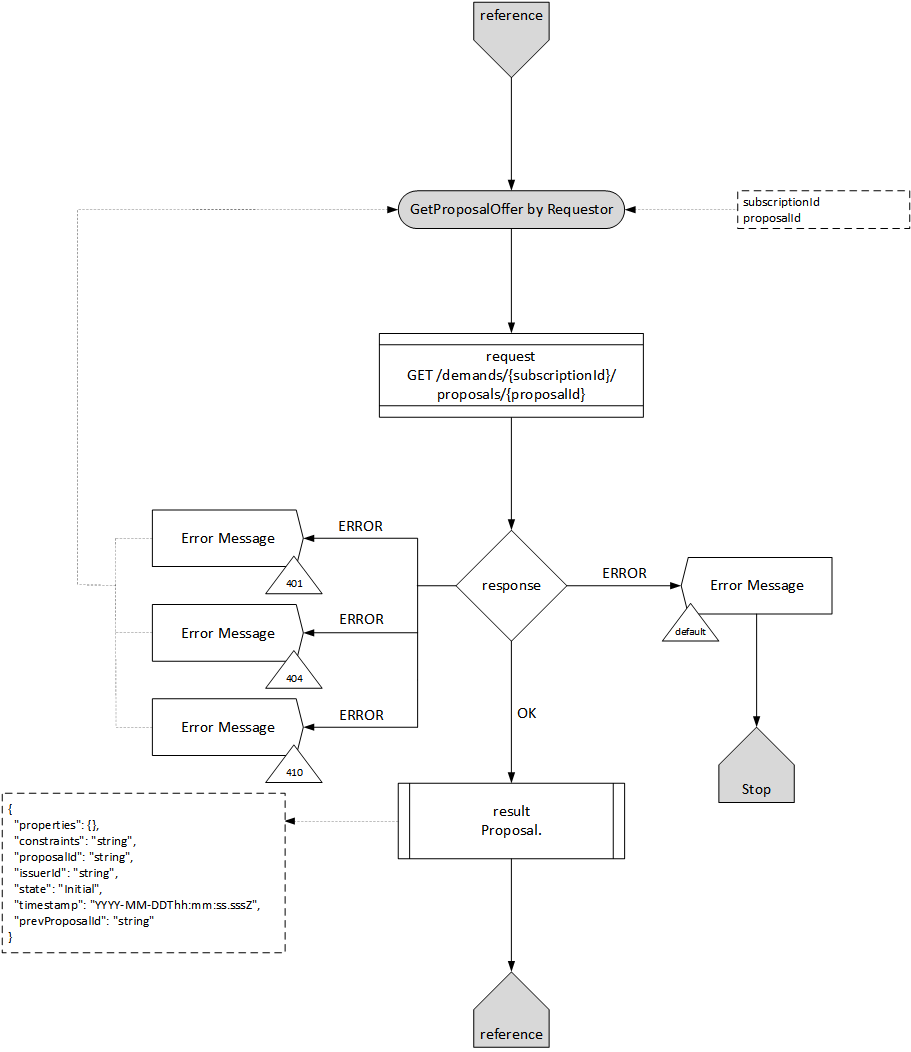
\includegraphics[width=12cm,height=12cm,angle=0]{./diag/Workflow/Market/GetProposalOffer-R-Workflow.png}
    \caption{Requestor Workflow Get Proposal Offer }
	\label{fig:GPO}
\end{figure}


\end{enumerate}

\newpage

\subsubsubsection{CounterProposalDemand Function}

\begin{enumerate}

\item Profile

\begin{enumerate}

\item Description

The CounterProposalDemand function is used to respond with bespoke Demand to received Offer. \\
It uses the POST /demands/\{subscriptionId\}/proposals/\{proposalId\} method.

\item Side

Requestor

\end{enumerate}

\item Request

\begin{enumerate}

\item Input

\begin{tcolorbox}[boxrule=0pt, frame empty]
\begin{verbatim}

subscriptionId
proposalId

\end{verbatim}
\end{tcolorbox}

Demand Object
\begin{tcolorbox}[boxrule=0pt, frame empty]
\begin{verbatim}
{
  "properties": {},
  "constraints": "string"
}
\end{verbatim}
\end{tcolorbox}

\begin{table}[H]
\footnotesize

\begin{center}
\begin{tabular}{|p{3cm}|l|p{3cm}|p{3cm}|p{4cm}|} 
\hline
\rowcolor{lightgray}	Name	& MO.	& Type	& Example & 	Description \\
\hline

subscriptionId	& M	& 	string			&		&	Subscription Identifier \\ 
\hline

proposalId		& M & 	string			&		&	Proposal Identifier \\
\hline	

properties		& M &	json or flat 	&		& Demand Properties		\\
\hline

constraints 	& M &	string			&		& Demand Constraints		\\
\hline

\end{tabular}
\end{center}

\end{table}

\item REST Method

\begin{tcolorbox}[boxrule=0pt, frame empty]
\begin{verbatim} 

POST /demands/{subscriptionId}/proposals/{proposalId}

\end{verbatim}
\end{tcolorbox}

\end{enumerate}

\item Response

\begin{table}[H]
\footnotesize

\begin{center}
\begin{tabular}{|c|l|} 
\hline
\rowcolor{lightgray}	Code 		& 	Description \\
\hline
201	 		&	Counter Proposal created.  \\
\hline
400			&	(400) Bad request	\\
\hline
404			&	(404) The specified resource was not found. \\
\hline
401			&	(401) Authorization information is missing or invalid. \\
\hline
410			&	Proposal rejected. \\
\hline
default		&	Unexpected error. \\
\hline
\end{tabular}
\end{center}

\end{table}

\item Result

\begin{tcolorbox}[boxrule=0pt, frame empty]
\begin{verbatim}
  proposalId
\end{verbatim}
\end{tcolorbox}

\begin{center}
\begin{tabular}{|p{3cm}|l|p{3cm}|p{3cm}|p{4cm}|} 
\hline
\rowcolor{lightgray}	Name	& MO.	& Type	& Example & 	Description \\
\hline

proposalId	&	&	string				&								& Proposal Identifier \\
\hline

\end{tabular}
\end{center}


\item Workflow

(Please see Figure ~\ref{fig:CPD} on page ~\pageref{fig:CPD}):

\begin{figure}[H]
    \centering
    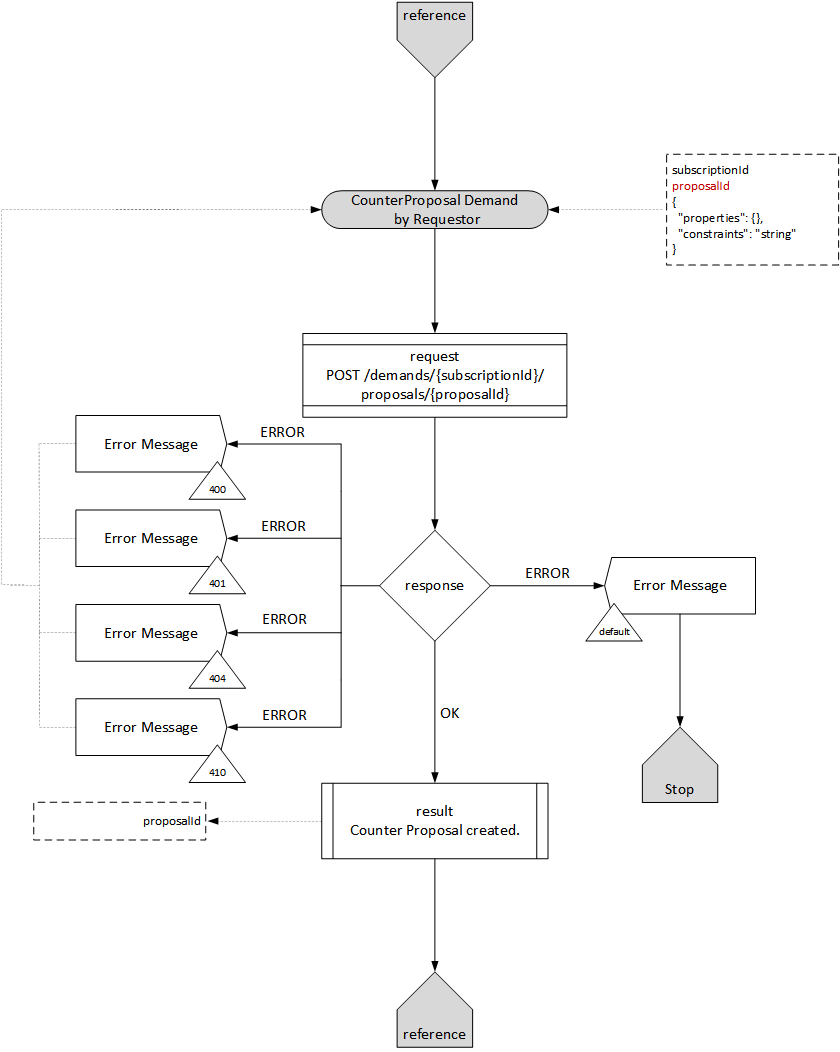
\includegraphics[width=12cm,height=12cm,angle=0]{./diag/Workflow/Market/CounterProposalDemand-R-Workflow.png}
    \caption{Requestor Workflow Counter Proposal Demand }
	\label{fig:CPD}
\end{figure}


\end{enumerate}

\newpage

\subsubsubsection{RejectProposalOffer Function}

\begin{enumerate}

\item Profile

\begin{enumerate}

\item Description

The RejectProposalOffer function is used to reject Proposal Offer. \\
It uses the POST /demands/\{subscriptionId\}/proposals/\{proposalId\}/reject method.

\item Side

Requestor

\end{enumerate}

\item Request

\begin{enumerate}

\item Input

\begin{tcolorbox}[boxrule=0pt, frame empty]
\begin{verbatim}

subscriptionId
proposalId

\end{verbatim}
\end{tcolorbox}

Object
\begin{tcolorbox}[boxrule=0pt, frame empty]
\begin{verbatim}
{
  "message": "string",
  "additionalProp1": {}
}
\end{verbatim}
\end{tcolorbox}

\begin{table}[H]
\footnotesize

\begin{center}
\begin{tabular}{|p{3cm}|l|p{3cm}|p{3cm}|p{4cm}|} 
\hline
\rowcolor{lightgray}	Name	& MO.	& Type	& Example & 	Description \\
\hline

subscriptionId		& M	& 	string			&		&	Subscription Identifier \\ 

\hline

proposalId			& M & 	string			&		&	Proposal Identifier \\

\hline	

message				& O &	string 			&		& 		\\

\hline

additionalProp1 	& O &	json			&		& 		\\

\hline

\end{tabular}
\end{center}

\end{table}

\item REST Method

\begin{tcolorbox}[boxrule=0pt, frame empty]
\begin{verbatim} 

POST /demands/{subscriptionId}/proposals/{proposalId}/reject

\end{verbatim}
\end{tcolorbox}

\end{enumerate}

\item Response

\begin{table}[H]
\footnotesize

\begin{center}
\begin{tabular}{|c|l|} 
\hline
\rowcolor{lightgray}	Code 		& 	Description \\
\hline
204	 		&	Proposal rejected.  \\
\hline
404			&	(404) The specified resource was not found. \\
\hline
401			&	(401) Authorization information is missing or invalid. \\
\hline
410			&	Proposal rejected. \\
\hline
default		&	Unexpected error. \\
\hline
\end{tabular}
\end{center}

\end{table}

\item Result

\begin{tcolorbox}[boxrule=0pt, frame empty]
\begin{verbatim}
  None
\end{verbatim}
\end{tcolorbox}

\item Workflow

(Please see Figure ~\ref{fig:RPO} on page ~\pageref{fig:RPO}):

\begin{figure}[H]
    \centering
    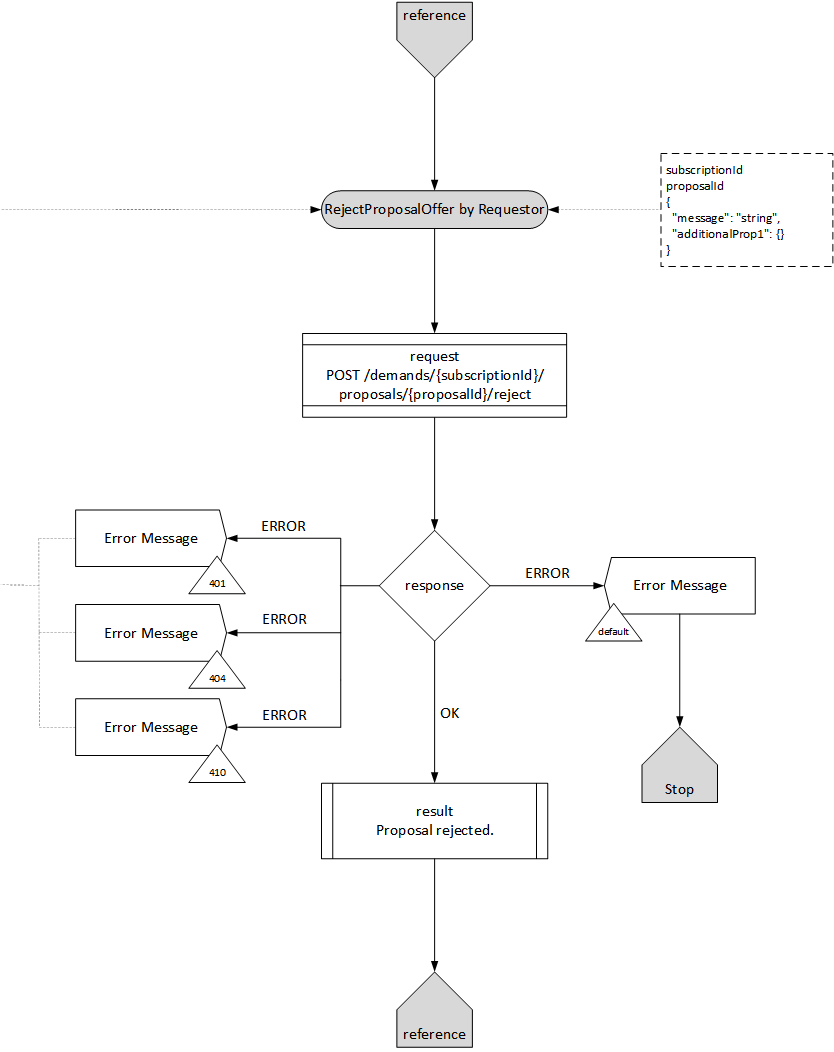
\includegraphics[width=12cm,height=12cm,angle=0]{./diag/Workflow/Market/RejectProposalOffer-R-Workflow.png}
    \caption{Requestor Workflow Reject Proposal Offer }
	\label{fig:RPO}
\end{figure}


\end{enumerate}

\newpage

\subsubsubsection{ListAgreements Function}

\begin{enumerate}

\item Profile

\begin{enumerate}

\item Description

The ListAgreements function is used to list Agreement objects with optional filters by the Requestor and Provider node. 
It uses the GET /agreements method.

\item Side

Both

\end{enumerate}

\item Request

\begin{enumerate}

\item Input

\begin{tcolorbox}[boxrule=0pt, frame empty]
\begin{verbatim}

appSessionId
state
afterTimestamp
beforeTimestamp

\end{verbatim}
\end{tcolorbox}

Object
\begin{tcolorbox}[boxrule=0pt, frame empty]
\begin{verbatim}
{
  "proposalId": "string",
  "validTo": "YYYY-MM-DDThh:mm:ss.sssZ"
}
\end{verbatim}
\end{tcolorbox}

\begin{table}[H]
\footnotesize

\begin{center}
\begin{tabular}{|p{3cm}|l|p{3cm}|p{3cm}|p{4cm}|} 
\hline
\rowcolor{lightgray}	Name	& MO.	& Type	& Example & 	Description \\
\hline

appSessionId	& O & 	string				&			& A correlation/session identifier used for querying events related to an action where this appSessionId has been specified \\
\hline

state			& O	& 	string(enum)		&	[Proposal, Pending, Cancelled, Rejected, Approved, Expired, Terminated]	&	State of an agreement \\ 
\hline

afterTimestamp	& O &	string(\$date-time)	&	YYYY-MM-DDThh:mm:ss.sssZ	&	Apply only to records created later than the specified timestamp \\
\hline

beforeTimestamp	& O &	string(\$date-time)	&	YYYY-MM-DDThh:mm:ss.sssZ	&	Apply only to records created before the specified timestamp \\
\hline

\end{tabular}
\end{center}

\end{table}

\item REST Method

\begin{tcolorbox}[boxrule=0pt, frame empty]
\begin{verbatim} 

GET /agreements

\end{verbatim}
\end{tcolorbox}

\end{enumerate}

\item Response

\begin{table}[H]
\footnotesize

\begin{center}
\begin{tabular}{|c|l|} 
\hline
\rowcolor{lightgray}	Code 		& 	Description \\
\hline
200	 		&	Result of listing agreements. \\
\hline
400			&	(400) Bad request \\
\hline
401			&	(401) Authorization information is missing or invalid. \\
\hline
default		&	Unexpected error. \\
\hline
\end{tabular}
\end{center}

\end{table}

\item Result

\begin{tcolorbox}[boxrule=0pt, frame empty]
\begin{verbatim}

[
  {
    "id": "string",
    "timestamp": "YYYY-MM-DDThh:mm:ss.sssZ",
    "approvedDate": "YYYY-MM-DDThh:mm:ss.sssZ",
    "role": "string"
  }
]

\end{verbatim}
\end{tcolorbox}

\begin{table}[H]
\footnotesize

\begin{center}
\begin{tabular}{|p{3cm}|l|p{3cm}|p{3cm}|p{4cm}|} 
\hline
\rowcolor{lightgray}	Name	& MO.	& Type	& Example & 	Description \\
\hline

id				& 	& 	string				&								&	Agreement Identyfier \\ 
\hline

timestamp		& 	& 	string(\$date-time)	&	YYYY-MM-DDThh:mm:ss.sssZ	&	 \\ 
\hline

approvedDate	& 	& 	string(\$date-time)	&	YYYY-MM-DDThh:mm:ss.sssZ	&	 \\ 
\hline

role			& 	& 	string				&								&	 \\ 
\hline

\end{tabular}
\end{center}

\end{table}


\item Workflow

(Please see Figure ~\ref{fig:BLA} on page ~\pageref{fig:BLA}):

\begin{figure}[H]
    \centering
    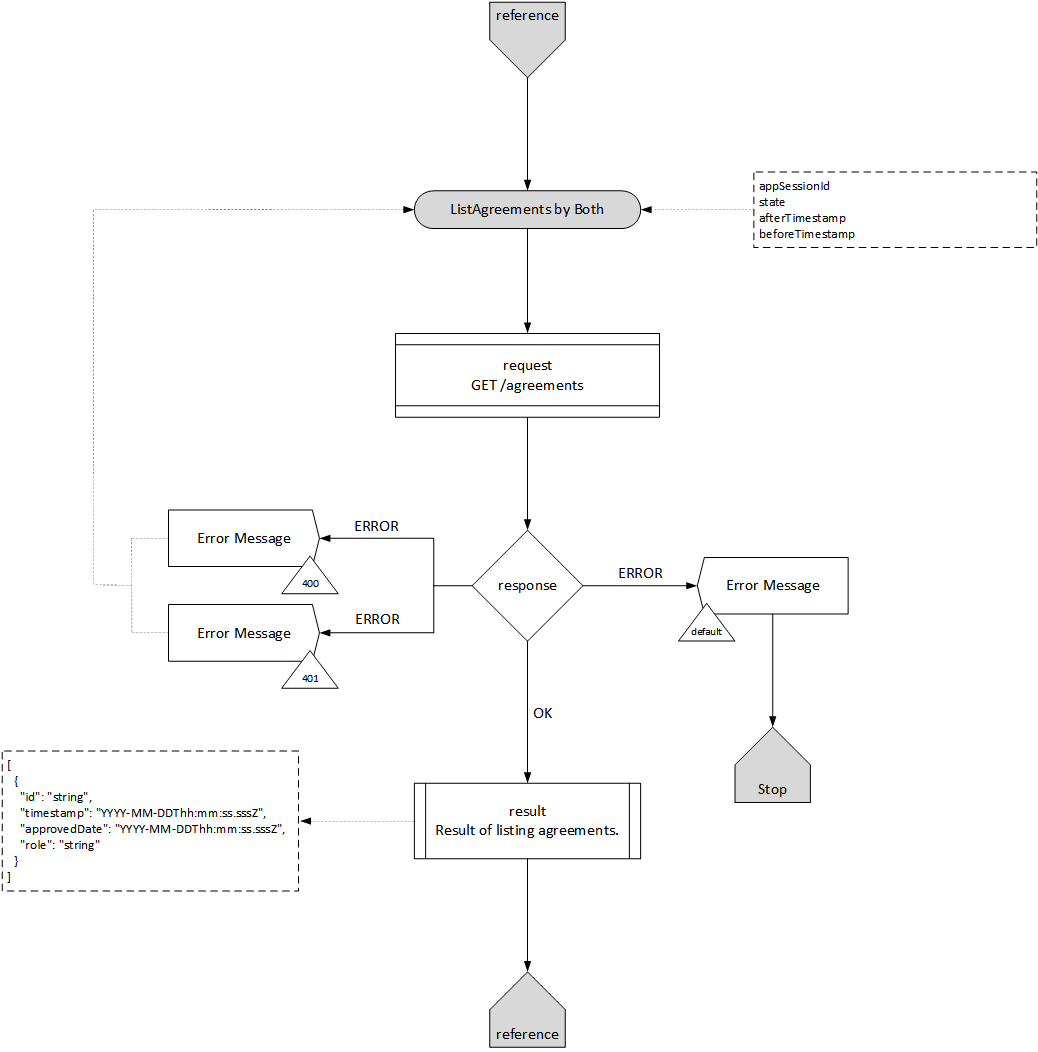
\includegraphics[width=11cm,height=11cm,angle=0]{./diag/Workflow/Market/ListAgreements-B-Workflow.png}
    \caption{Both Workflow List Agreements }
	\label{fig:BLA}
\end{figure}

\end{enumerate}

\newpage

\subsubsubsection{GetAgreement Function}

\begin{enumerate}

\item Profile

\begin{enumerate}

\item Description

The GetAgreement function is used to fetch Agreement objects with given agreementId by the Requestor and Provider node. 
It uses the GET /agreements/\{agreementId\} method.

\item Side

Both

\end{enumerate}

\item Request

\begin{enumerate}

\item Input

\begin{tcolorbox}[boxrule=0pt, frame empty]
\begin{verbatim}

agreementId

\end{verbatim}
\end{tcolorbox}

%Object
%\begin{tcolorbox}[boxrule=0pt, frame empty]
%\begin{verbatim}
%{
%  "proposalId": "string",
%  "validTo": "YYYY-MM-DDThh:mm:ss.sssZ"
%}
%\end{verbatim}
%\end{tcolorbox}

\begin{table}[H]
\footnotesize

\begin{center}
\begin{tabular}{|p{3cm}|l|p{3cm}|p{3cm}|p{4cm}|} 
\hline
\rowcolor{lightgray}	Name	& MO.	& Type	& Example & 	Description \\
\hline

agreementId	& M & 	string				&			& Agreement Identifier \\
\hline

\end{tabular}
\end{center}

\end{table}

\item REST Method

\begin{tcolorbox}[boxrule=0pt, frame empty]
\begin{verbatim} 

GET /agreements/agreementId

\end{verbatim}
\end{tcolorbox}

\end{enumerate}

\item Response

\begin{table}[H]
\footnotesize

\begin{center}
\begin{tabular}{|c|l|} 
\hline
\rowcolor{lightgray}	Code 		& 	Description \\
\hline
200	 		&	Agreement. \\
\hline
404			&	(404) The specified resource was not found. \\
\hline
401			&	(401) Authorization information is missing or invalid. \\
\hline
default		&	Unexpected error. \\
\hline
\end{tabular}
\end{center}

\end{table}

\item Result

\begin{tcolorbox}[boxrule=0pt, frame empty]
\begin{verbatim}

{
  "agreementId": "string",
  "demand": {
    "properties": {},
    "constraints": "string",
    "demandId": "string",
    "requestorId": "string",
    "timestamp": "YYYY-MM-DDThh-MM-DDThh:mm:ss.sssZ"
  },
  "offer": {
    "properties": {},
    "constraints": "string",
    "offerId": "string",
    "providerId": "string",
    "timestamp": "YYYY-MM-DDThh-MM-DDThh:mm:ss.sssZ"
  },
  "validTo": "YYYY-MM-DDThh-MM-DDThh:mm:ss.sssZ",
  "approvedDate": "YYYY-MM-DDThh-MM-DDThh:mm:ss.sssZ",
  "state": "Proposal",
  "timestamp": "YYYY-MM-DDThh-MM-DDThh:mm:ss.sssZ",
  "appSessionId": "string",
  "proposedSignature": "string",
  "approvedSignature": "string",
  "committedSignature": "string"
}

\end{verbatim}
\end{tcolorbox}

\begin{table}[H]
\footnotesize

\begin{center}
\begin{tabular}{|p{3cm}|l|p{3cm}|p{3cm}|p{4cm}|} 
\hline
\rowcolor{lightgray}	Name	& MO.	& Type	& Example & 	Description \\
\hline

agreementId				& 	& 	string				&		&	Agreement Identyfier \\ 
\hline

demand.properties		&	&	json or flat		&		& 	Demand Properties \\
\hline

demand.constraints		&	&	string				&		&	Demand Constraints \\	
\hline

demand.demandId			&	&	string				&		&	Demand Identifier \\
\hline 		

demand.requestorId		&	&	string 				&		&	Requestor Node Identifier \\
\hline

demand.timestamp		& 	& 	string(\$date-time)	&	YYYY-MM-DDThh:mm:ss.sssZ	&	 \\ 
\hline

offer.properties		&	&	json or flat		&		& 	Offer Properties \\
\hline

offer.constraints		&	&	string				&		&	Offer Constraints \\	
\hline

offer.offerId			&	&	string				&		&	Offer Identifier \\
\hline 		

offer.providerId		&	&	string 				&		&	Provider Node Identifier \\
\hline

offer.timestamp		& 	& 	string(\$date-time)	&	YYYY-MM-DDThh:mm:ss.sssZ	&	 \\ 
\hline

validTo			& 	& 	string(\$date-time)	&	YYYY-MM-DDThh:mm:ss.sssZ	&	 \\ 
\hline

approvedDate	& 	& 	string(\$date-time)	&	YYYY-MM-DDThh:mm:ss.sssZ	&	 \\ 
\hline

state			& 	& 	string(enum)		&	[ Proposal, Pending, Cancelled, Rejected, Approved, Expired, Terminated ]	& Agreement State	\\ 
\hline

timestamp		& 	& 	string(\$date-time)	&	YYYY-MM-DDThh:mm:ss.sssZ	&	 \\ 
\hline

appSessionId	&	&	string 				&			&	AppSessionId \\
\hline

proposedSignature &		& string 			&			&	Proposed Signature \\
\hline

approvedSignature &		&  string			&			&  Approved Signature \\
\hline  
  
committedSignature &	& 	string			&			&	Committed Signature \\
\hline

\end{tabular}
\end{center}

\end{table}

\item Workflow

(Please see Figure ~\ref{fig:BGA} on page ~\pageref{fig:BGA}):

\begin{figure}[H]
    \centering
    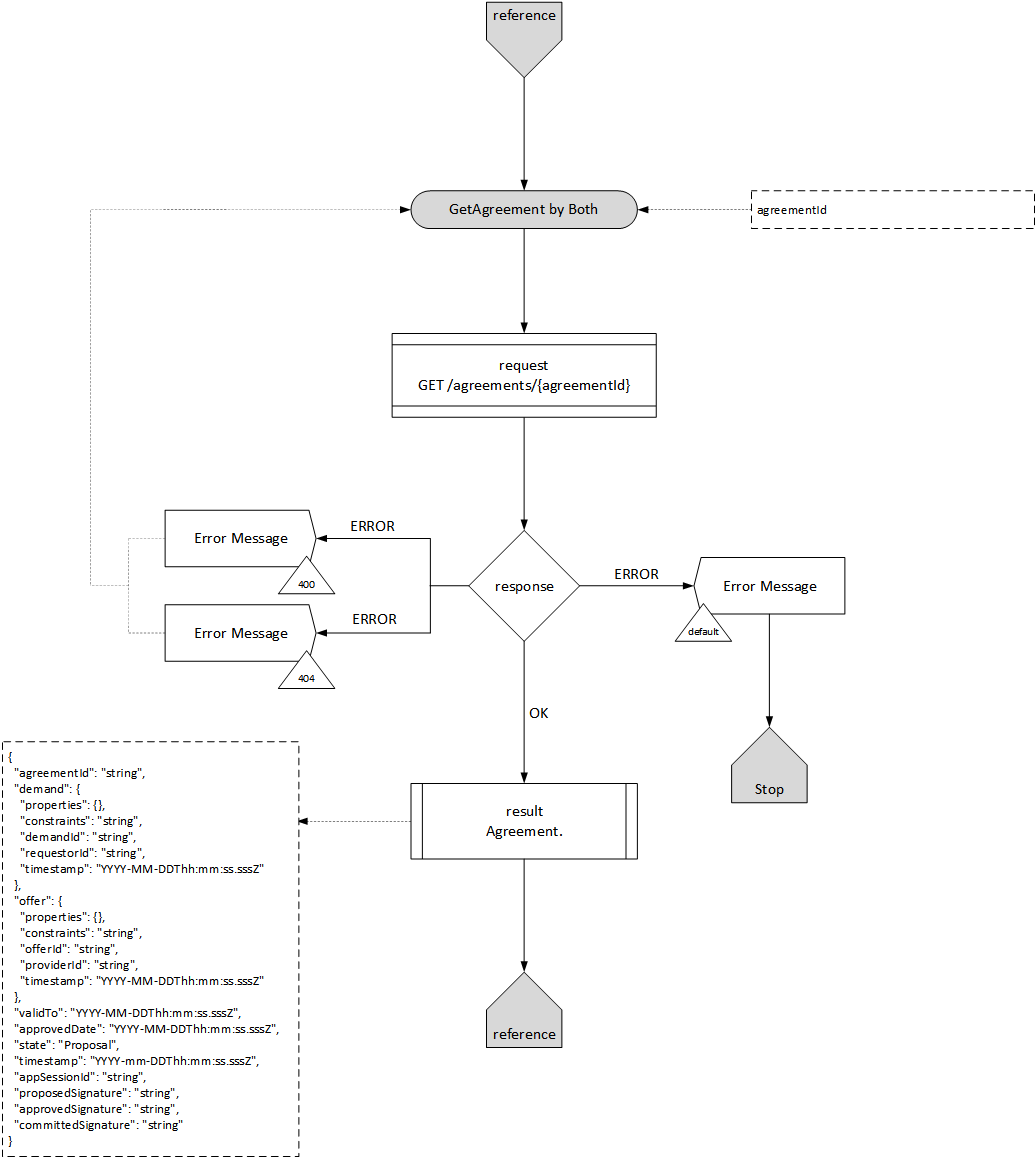
\includegraphics[width=11cm,height=11cm,angle=0]{./diag/Workflow/Market/GetAgreement-B-Workflow.png}
    \caption{Both Workflow Get Agreement }
	\label{fig:BGA}
\end{figure}

\end{enumerate}

\newpage

% AgreementEvents
\subsubsubsection{CollectAgreementEvents Function}

\begin{enumerate}

\item Profile

\begin{enumerate}

\item Description

The CollectAgreementEvents function is used to collect events related to an Agreement objects with optional filters by the Requestor and Provider node. 
It uses the GET /agreementEvents method.

\item Side

Both

\end{enumerate}

\item Request

\begin{enumerate}

\item Input

\begin{tcolorbox}[boxrule=0pt, frame empty]
\begin{verbatim}

appSessionId
maxEvents
afterTimestamp
timeout

\end{verbatim}
\end{tcolorbox}

%Object
%\begin{tcolorbox}[boxrule=0pt, frame empty]
%\begin{verbatim}
%{
%  "proposalId": "string",
%  "validTo": "YYYY-MM-DDThh:mm:ss.sssZ"
%}
%\end{verbatim}
%\end{tcolorbox}

\begin{table}[H]
\footnotesize

\begin{center}
\begin{tabular}{|p{3cm}|l|p{3cm}|p{3cm}|p{4cm}|} 
\hline
\rowcolor{lightgray}	Name	& MO.	& Type	& Example & 	Description \\
\hline

appSessionId	& O & 	string				&			& A correlation/session identifier used for querying events related to an action where this appSessionId has been specified \\
\hline

maxEvents			& O	& 	integer(\$int32)		&	10	&	Maximum number of events that server should return at once. \\ 
\hline

afterTimestamp	& O &	string(\$date-time)	&	YYYY-MM-DDThh:mm:ss.sssZ	&	Apply only to records created later than the specified timestamp \\
\hline

timeout	& O &	number(\$float)	&	5	&	Timeout used in long-polling calls (in seconds). 
											How many seconds server should wait for response containing new events 
											(0.0 means it should return immediately if there are no events) \\
\hline

\end{tabular}
\end{center}

\end{table}

\item REST Method

\begin{tcolorbox}[boxrule=0pt, frame empty]
\begin{verbatim} 

GET /agreementEvents

\end{verbatim}
\end{tcolorbox}

\end{enumerate}

\item Response

\begin{table}[H]
\footnotesize

\begin{center}
\begin{tabular}{|c|l|} 
\hline
\rowcolor{lightgray}	Code 		& 	Description \\
\hline
200	 		&	Agreement-related event list. \\
\hline
400			&	(400) Bad request \\
\hline
401			&	(401) Authorization information is missing or invalid. \\
\hline
default		&	Unexpected error. \\
\hline
\end{tabular}
\end{center}

\end{table}

\item Result

\begin{tcolorbox}[boxrule=0pt, frame empty]
\begin{verbatim}

[
  {
    "eventType": "string",
    "eventDate": "YYYY-MM-DDThh:mm:ss.sssZ",
    "agreementId": "string"
  }
]

\end{verbatim}
\end{tcolorbox}

\begin{table}[H]
\footnotesize

\begin{center}
\begin{tabular}{|p{3cm}|l|p{3cm}|p{3cm}|p{4cm}|} 
\hline
\rowcolor{lightgray}	Name	& MO.	& Type	& Example & 	Description \\
\hline

agreementId		& 	& 	string				&						&	Agreement Identyfier \\ 
\hline

eventDate		& 	& 	string(\$date-time)	&	YYYY-MM-DDThh:mm:ss.sssZ	&	 \\ 
\hline

eventType		& 	& 	string(enum)		&	[AgreementApprovedEvent, AgreementRejectedEvent, AgreementCancelledEvent, AgreementTerminatedEvent] &	Event Type \\ 
\hline

\end{tabular}
\end{center}

\end{table}

\item Workflow

(Please see Figure ~\ref{fig:CAE} on page ~\pageref{fig:CAE}):

\begin{figure}[H]
    \centering
    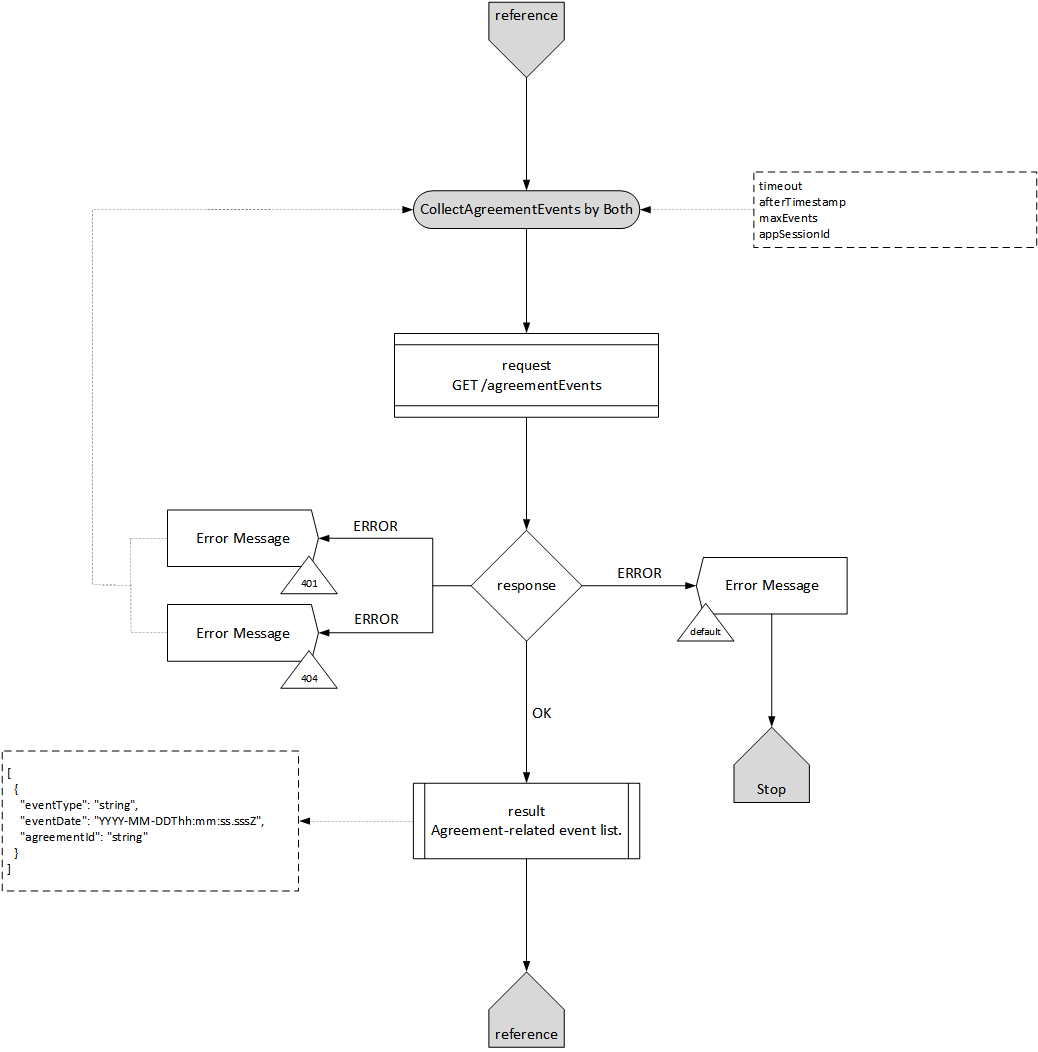
\includegraphics[width=11cm,height=11cm,angle=0]{./diag/Workflow/Market/CollectAgreementEvents-B-Workflow.png}
    \caption{Both Workflow Collect Agreement Events }
	\label{fig:CAE}
\end{figure}

\end{enumerate}

\newpage

% TerminateAgreement
\subsubsubsection{TerminateAgreement Function}

\begin{enumerate}

\item Profile

\begin{enumerate}

\item Description

The TerminateAgreement function is used to terminate approved Agreement objects by the Requestor and Provider node. 
It uses the POST /agreements/\{agreementId\}/terminate method.

\item Side

Both

\end{enumerate}

\item Request

\begin{enumerate}

\item Input

\begin{tcolorbox}[boxrule=0pt, frame empty]
\begin{verbatim}

agreementId

\end{verbatim}
\end{tcolorbox}

Object
\begin{tcolorbox}[boxrule=0pt, frame empty]
\begin{verbatim}
{
  "message": "string",
  "additionalProp1": {}
}
\end{verbatim}
\end{tcolorbox}

\begin{table}[H]
\footnotesize

\begin{center}
\begin{tabular}{|p{3cm}|l|p{3cm}|p{3cm}|p{4cm}|} 
\hline
\rowcolor{lightgray}	Name	& MO.	& Type	& Example & 	Description \\
\hline

agreementId		& M & 	string				&		& 	Agreement Identifier \\
\hline

message			& O	& 	string				&		&	 	\\ 
\hline

additionalProp1	& O &	json				&		&		\\
\hline

\end{tabular}
\end{center}

\end{table}

\item REST Method

\begin{tcolorbox}[boxrule=0pt, frame empty]
\begin{verbatim} 

POST /agreements/{agreementId}/terminate

\end{verbatim}
\end{tcolorbox}

\end{enumerate}

\item Response

\begin{table}[H]
\footnotesize

\begin{center}
\begin{tabular}{|c|l|} 
\hline
\rowcolor{lightgray}	Code 		& 	Description \\
\hline
204	 		&	Agreement terminated. \\
\hline
404			&	(404) The specified resource was not found. \\
\hline
401			&	(401) Authorization information is missing or invalid. \\
\hline
409			&	(409) Conflict. \\
\hline
410			&	(410) Gone \\
\hline
default		&	Unexpected error. \\
\hline
\end{tabular}
\end{center}

\end{table}

\item Result

\begin{tcolorbox}[boxrule=0pt, frame empty]
\begin{verbatim}

None

\end{verbatim}
\end{tcolorbox}

%\begin{center}
%\begin{tabular}{|p{3cm}|l|p{3cm}|p{3cm}|p{4cm}|} 
%\hline
%\rowcolor{lightgray}	Name	& MO.	& Type	& Example & 	Description \\
%\hline
%agreementId		& 	& 	string				&						&	Agreement Identyfier \\ 
%\hline
%eventDate		& 	& 	string(\$date-time)	&	YYYY-MM-DDThh:mm:ss.sssZ	&	 \\ 
%\hline
%eventType		& 	& 	string(enum)		&	 &	Event Type \\ 
%\hline
%\end{tabular}
%\end{center}

\item Workflow

(Please see Figure ~\ref{fig:BTA} on page ~\pageref{fig:BTA}):

\begin{figure}[H]
    \centering
    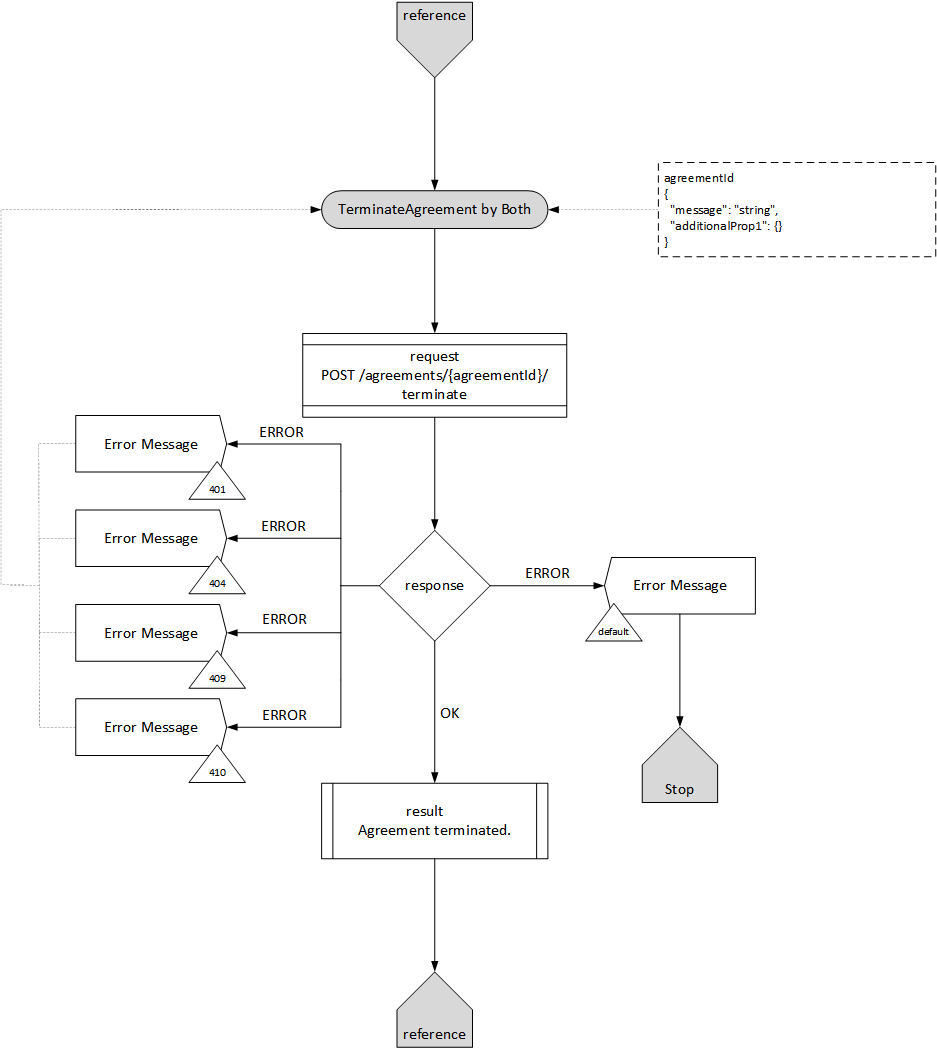
\includegraphics[width=11cm,height=11cm,angle=0]{./diag/Workflow/Market/TerminateAgreement-B-Workflow.png}
    \caption{Both Workflow Terminate Agreement  }
	\label{fig:BTA}
\end{figure}

\end{enumerate}

\newpage

% ReasonTerminateAgreement
\subsubsubsection{ReasonTerminateAgreement Function}

\begin{enumerate}

\item Profile

\begin{enumerate}

\item Description

The ReasonTerminateAgreement function is used to get termination reason reported when terminateAgreement was called. 
This method is used by the Requestor and Provider node. It uses the POST /agreements/\{agreementId\}/terminate/reason method.

\item Side

Both

\end{enumerate}

\item Request

\begin{enumerate}

\item Input

\begin{tcolorbox}[boxrule=0pt, frame empty]
\begin{verbatim}

agreementId

\end{verbatim}
\end{tcolorbox}

%Object
%\begin{tcolorbox}[boxrule=0pt, frame empty]
%\begin{verbatim}
%agreementId
%
%\end{verbatim}
%\end{tcolorbox}

\begin{table}[H]
\footnotesize

\begin{center}
\begin{tabular}{|p{3cm}|l|p{3cm}|p{3cm}|p{4cm}|} 
\hline
\rowcolor{lightgray}	Name	& MO.	& Type	& Example & 	Description \\
\hline
agreementId		& M & 	string				&		& 	Agreement Identifier \\
\hline
\end{tabular}
\end{center}

\end{table}

\item REST Method

\begin{tcolorbox}[boxrule=0pt, frame empty]
\begin{verbatim} 

POST /agreements/{agreementId}/terminate/reason

\end{verbatim}
\end{tcolorbox}

\end{enumerate}

\item Response

\begin{table}[H]
\footnotesize

\begin{center}
\begin{tabular}{|c|l|} 
\hline
\rowcolor{lightgray}	Code 		& 	Description \\
\hline
200	 		&	Agreement termination reason. \\
\hline
404			&	(404) The specified resource was not found. \\
\hline
401			&	(401) Authorization information is missing or invalid. \\
\hline
400			&	(400) Bad request \\
\hline
default		&	Unexpected error. \\
\hline
\end{tabular}
\end{center}

\end{table}

\item Result

\begin{tcolorbox}[boxrule=0pt, frame empty]
\begin{verbatim}

{
  "eventType": "string",
  "eventDate": "YYYY-MM-DDThh:mm:ss.sssZ",
  "agreementId": "string",
  "terminator": "Requestor",
  "signature": "string",
  "reason": {
    "message": "string",
    "additionalProp1": {}
  }
}

\end{verbatim}
\end{tcolorbox}

\begin{table}[H]
\footnotesize

\begin{center}
\begin{tabular}{|p{3cm}|l|p{3cm}|p{3cm}|p{4cm}|} 
\hline
\rowcolor{lightgray}	Name	& MO.	& Type	& Example & 	Description \\
\hline
agreementId		& 	& 	string				&								&	Agreement Identyfier \\ 
\hline
eventDate		& 	& 	string(\$date-time)	&	YYYY-MM-DDThh:mm:ss.sssZ	&	 \\ 
\hline
eventType		& 	& 	string(enum)		&	[AgreementApprovedEvent, AgreementRejectedEvent, AgreementCancelledEvent, AgreementTerminatedEvent] &	Event Type \\ 
\hline
terminator 		&	&	enum 				& [Requestor, Provider]			&				\\
\hline
signature 		&	&	string 				&								&				\\
\hline
reason.message 	&	&	string 				&								&				\\
\hline
reason.additionalProp1	&	&	json 			&								&				\\
\hline

\end{tabular}
\end{center}

\end{table}

\item Workflow

(Please see Figure ~\ref{fig:BRTA} on page ~\pageref{fig:BRTA}):

\begin{figure}[H]
    \centering
    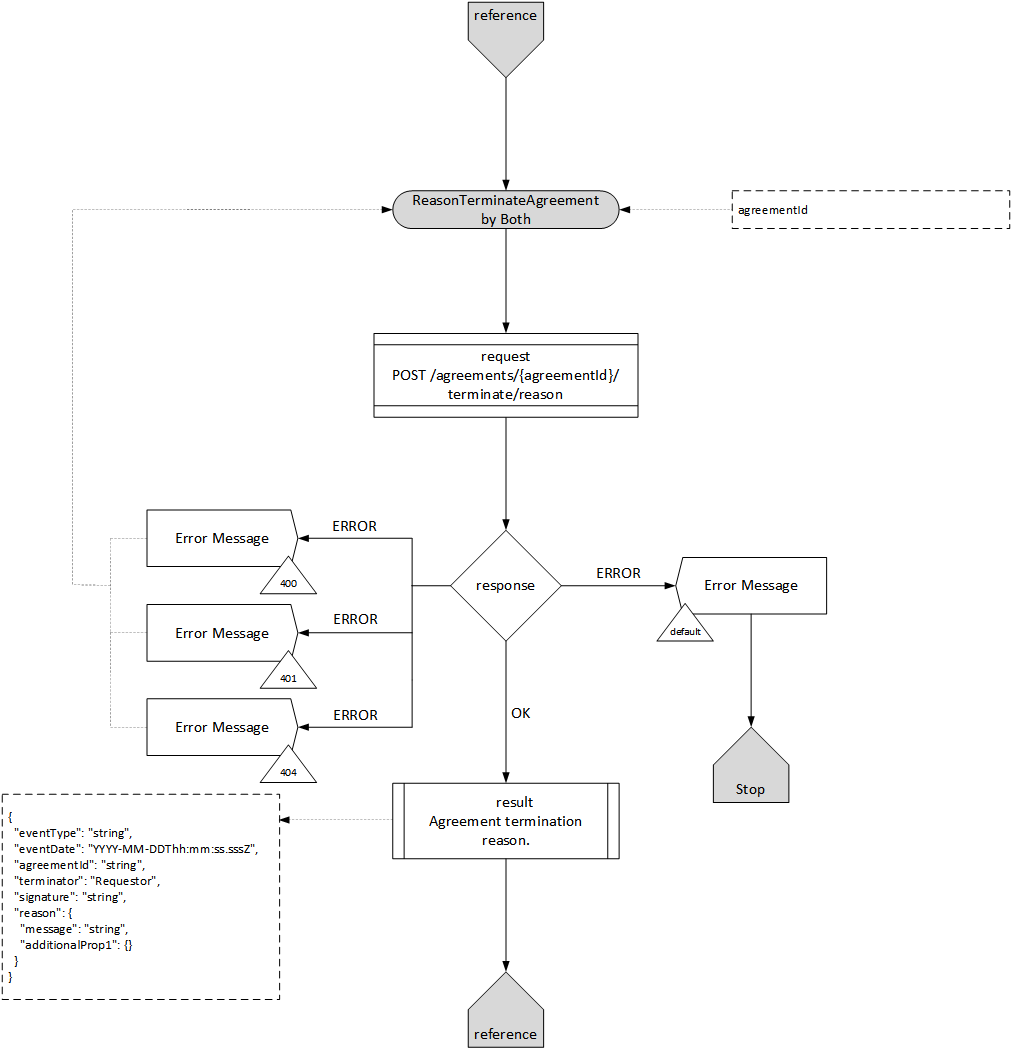
\includegraphics[width=11cm,height=11cm,angle=0]{./diag/Workflow/Market/ReasonTerminateAgreement-B-Workflow.png}
    \caption{Both Workflow Reason Terminate Agreement  }
	\label{fig:BRTA}
\end{figure}

\end{enumerate}

\newpage

% ConfirmAgreement

\subsubsubsection{ConfirmAgreement Function}

\begin{enumerate}

\item Profile

\begin{enumerate}

\item Description

The ConfirmAgreement function is used to send Agreement proposal object to the Provider by the Requestor node. 
It uses the POST /agreements/\{agreementId\}/confirm method.

\item Side

Requestor

\end{enumerate}

\item Request

\begin{enumerate}

\item Input

\begin{tcolorbox}[boxrule=0pt, frame empty]
\begin{verbatim}

agreementId
appSessionId

\end{verbatim}
\end{tcolorbox}

%Object
%\begin{tcolorbox}[boxrule=0pt, frame empty]
%\begin{verbatim}
%{
%  "message": "string",
%  "additionalProp1": {}
%}
%\end{verbatim}
%\end{tcolorbox}

\begin{table}[H]
\footnotesize

\begin{center}
\begin{tabular}{|p{3cm}|l|p{3cm}|p{3cm}|p{4cm}|} 
\hline
\rowcolor{lightgray}	Name	& MO.	& Type	& Example & 	Description \\
\hline

agreementId		& M & 	string				&		& 	Agreement Identifier \\
\hline

appSessionId	& O	& 	string				&		&	A correlation/session identifier used for querying events related to an action where this appSessionId has been specified 	\\ 
\hline

\end{tabular}
\end{center}

\end{table}

\item REST Method

\begin{tcolorbox}[boxrule=0pt, frame empty]
\begin{verbatim} 

POST /agreements/{agreementId}/confirm

\end{verbatim}
\end{tcolorbox}

\end{enumerate}

\item Response

\begin{table}[H]
\footnotesize

\begin{center}
\begin{tabular}{|c|l|} 
\hline
\rowcolor{lightgray}	Code 		& 	Description \\
\hline
204	 		&	Agreement confirmed. \\
\hline
404			&	(404) The specified resource was not found. \\
\hline
401			&	(401) Authorization information is missing or invalid. \\
\hline
410			&	(410) Gone \\
\hline
default		&	Unexpected error. \\
\hline
\end{tabular}
\end{center}

\end{table}

\item Result

\begin{tcolorbox}[boxrule=0pt, frame empty]
\begin{verbatim}

None

\end{verbatim}
\end{tcolorbox}

%\begin{center}
%\begin{tabular}{|p{3cm}|l|p{3cm}|p{3cm}|p{4cm}|} 
%\hline
%\rowcolor{lightgray}	Name	& MO.	& Type	& Example & 	Description \\
%\hline
%agreementId		& 	& 	string				&						&	Agreement Identyfier \\ 
%\hline
%eventDate		& 	& 	string(\$date-time)	&	YYYY-MM-DDThh:mm:ss.sssZ	&	 \\ 
%\hline
%eventType		& 	& 	string(enum)		&	 &	Event Type \\ 
%\hline
%\end{tabular}
%\end{center}

\item Workflow

(Please see Figure ~\ref{fig:RCA} on page ~\pageref{fig:RCA}):

\begin{figure}[H]
    \centering
    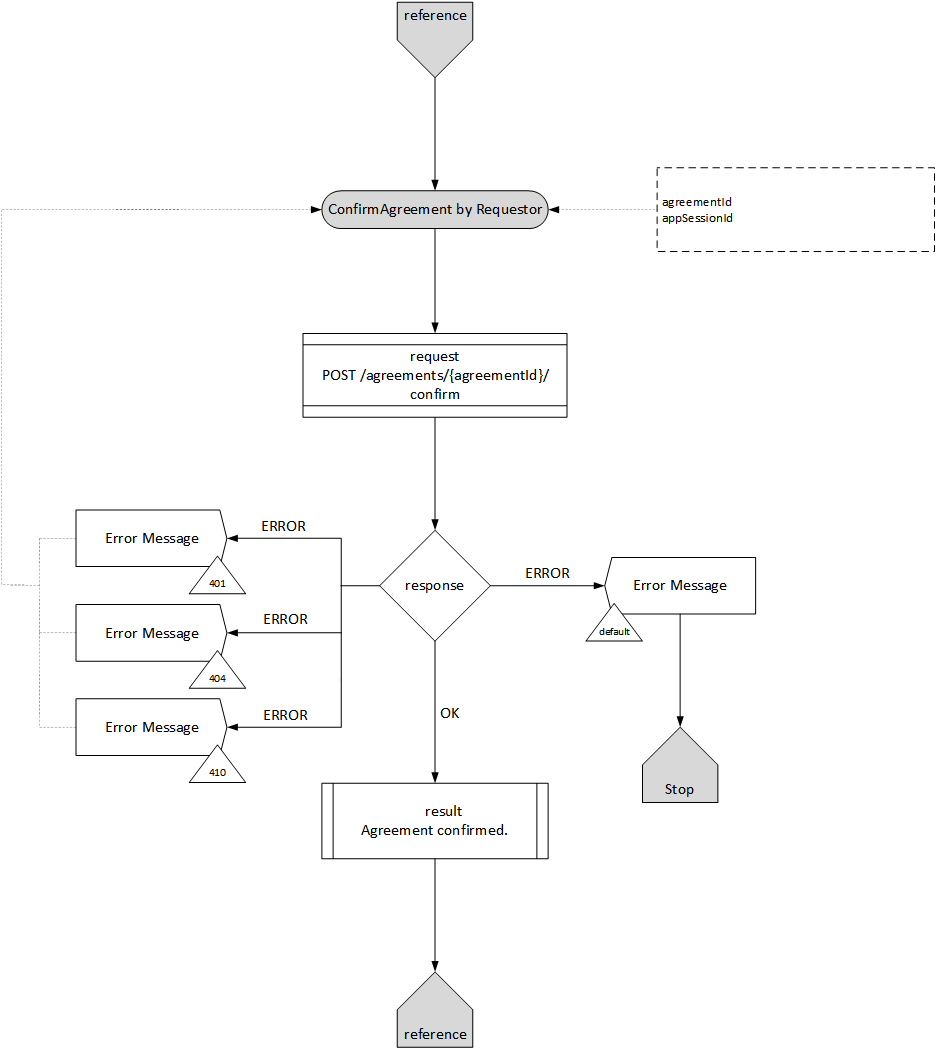
\includegraphics[width=11cm,height=11cm,angle=0]{./diag/Workflow/Market/ConfirmAgreement-R-Workflow.png}
    \caption{Requestor Workflow Confirm Agreement  }
	\label{fig:RCA}
\end{figure}

\end{enumerate}

\newpage

% CancelAgreement

\subsubsubsection{CancelAgreement Function}

\begin{enumerate}

\item Profile

\begin{enumerate}

\item Description

The CancelAgreement function is used to cancel Agreement object by the Requestor node. 
It uses the POST /agreements/\{agreementId\}/cancel method.

\item Side

Requestor

\end{enumerate}

\item Request

\begin{enumerate}

\item Input

\begin{tcolorbox}[boxrule=0pt, frame empty]
\begin{verbatim}

agreementId
appSessionId

\end{verbatim}
\end{tcolorbox}

Object
\begin{tcolorbox}[boxrule=0pt, frame empty]
\begin{verbatim}
{
  "message": "string",
  "additionalProp1": {}
}
\end{verbatim}
\end{tcolorbox}

\begin{table}[H]
\footnotesize

\begin{center}
\begin{tabular}{|p{3cm}|l|p{3cm}|p{3cm}|p{4cm}|} 
\hline
\rowcolor{lightgray}	Name	& MO.	& Type	& Example & 	Description \\
\hline

agreementId		& M & 	string				&		& 	Agreement Identifier \\
\hline

message 		& O	& 	string				&		&	 	\\ 
\hline

additionalProp1 & O	& 	json				&		&	 	\\ 
\hline

\end{tabular}
\end{center}

\end{table}

\item REST Method

\begin{tcolorbox}[boxrule=0pt, frame empty]
\begin{verbatim} 

POST /agreements/{agreementId}/cancel

\end{verbatim}
\end{tcolorbox}

\end{enumerate}

\item Response

\begin{table}[H]
\footnotesize

\begin{center}
\begin{tabular}{|c|l|} 
\hline
\rowcolor{lightgray}	Code 		& 	Description \\
\hline
204	 		&	Agreement cancelled. \\
\hline
404			&	(404) The specified resource was not found. \\
\hline
401			&	(401) Authorization information is missing or invalid. \\
\hline
410			&	(410) Gone \\
\hline
default		&	Unexpected error. \\
\hline
\end{tabular}
\end{center}

\end{table}

\item Result

\begin{tcolorbox}[boxrule=0pt, frame empty]
\begin{verbatim}

None

\end{verbatim}
\end{tcolorbox}

%\begin{center}
%\begin{tabular}{|p{3cm}|l|p{3cm}|p{3cm}|p{4cm}|} 
%\hline
%\rowcolor{lightgray}	Name	& MO.	& Type	& Example & 	Description \\
%\hline
%agreementId		& 	& 	string				&						&	Agreement Identyfier \\ 
%\hline
%eventDate		& 	& 	string(\$date-time)	&	YYYY-MM-DDThh:mm:ss.sssZ	&	 \\ 
%\hline
%eventType		& 	& 	string(enum)		&	 &	Event Type \\ 
%\hline
%\end{tabular}
%\end{center}

\item Workflow

(Please see Figure ~\ref{fig:RCCA} on page ~\pageref{fig:RCCA}):

\begin{figure}[H]
    \centering
    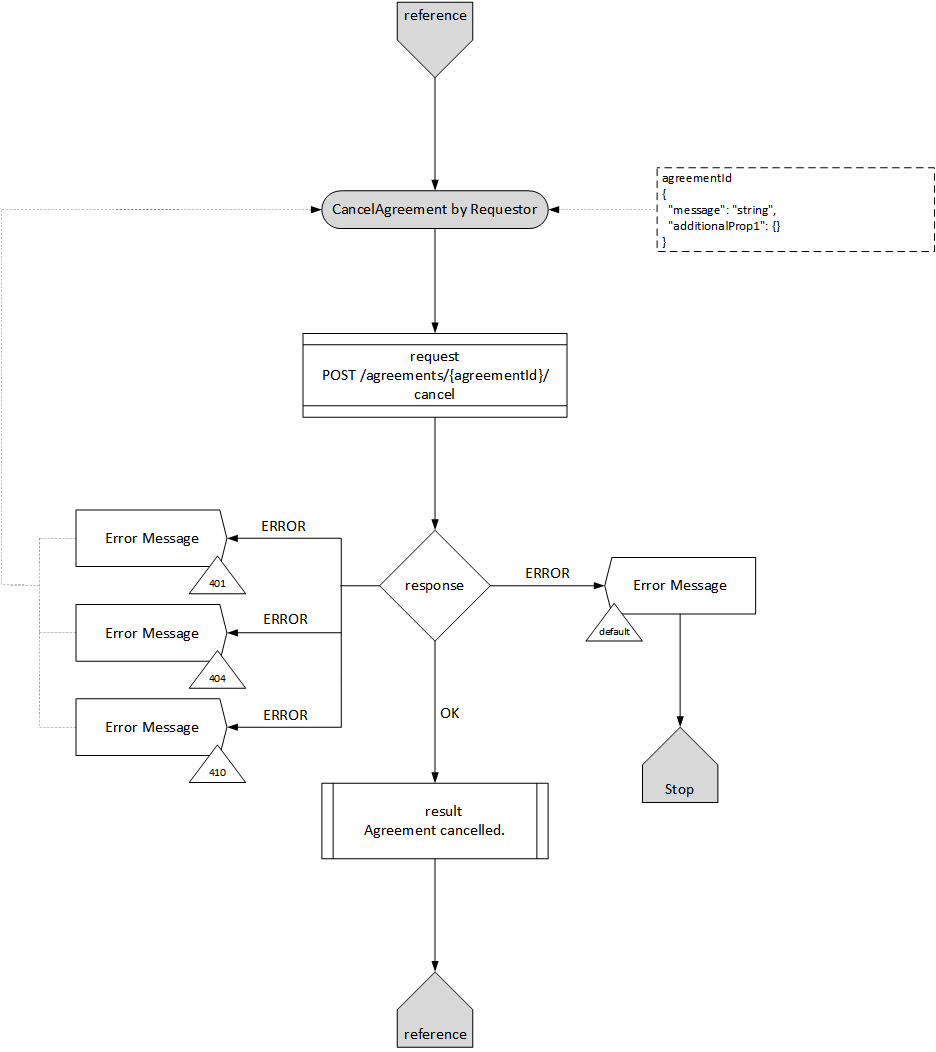
\includegraphics[width=11cm,height=11cm,angle=0]{./diag/Workflow/Market/CancelAgreement-R-Workflow.png}
    \caption{Requestor Workflow Cancel Agreement  }
	\label{fig:RCCA}
\end{figure}

\end{enumerate}

\newpage

% WaitAgreement WaitForApproval

\subsubsubsection{WaitForApproval Function}

\begin{enumerate}

\item Profile

\begin{enumerate}

\item Description

The WaitForApproval function is used to wait for Agreement approval by the Provider. This method is used by the Requestor node. 
It uses the POST /agreements/\{agreementId\}/wait method.

\item Side

Requestor

\end{enumerate}

\item Request

\begin{enumerate}

\item Input

\begin{tcolorbox}[boxrule=0pt, frame empty]
\begin{verbatim}

agreementId
timeout

\end{verbatim}
\end{tcolorbox}

%Object
%\begin{tcolorbox}[boxrule=0pt, frame empty]
%\begin{verbatim}
%{
%  "message": "string",
%  "additionalProp1": {}
%}
%\end{verbatim}
%\end{tcolorbox}

\begin{table}[H]
\footnotesize

\begin{center}
\begin{tabular}{|p{3cm}|l|p{3cm}|p{3cm}|p{4cm}|} 
\hline
\rowcolor{lightgray}	Name	& MO.	& Type	& Example & 	Description \\
\hline

agreementId		& M & 	string				&		& 	Agreement Identifier \\
\hline

timeout 		& O	& 	number(\$float)				&	5	&	Timeout used in blocking calls waiting for eg. acknowledgement. 
																How many seconds server should wait for response/acknowledgement of an action 
																(0.0 means it should wait for other party's response indefinitely)	\\ 
\hline

\end{tabular}
\end{center}

\end{table}

\item REST Method

\begin{tcolorbox}[boxrule=0pt, frame empty]
\begin{verbatim} 

POST /agreements/{agreementId}/wait

\end{verbatim}
\end{tcolorbox}

\end{enumerate}

\item Response

\begin{table}[H]
\footnotesize

\begin{center}
\begin{tabular}{|c|l|} 
\hline
\rowcolor{lightgray}	Code 		& 	Description \\
\hline
204	 		&	Agreement approved by the Provider. \\
\hline
404			&	(404) The specified resource was not found. \\
\hline
401			&	(401) Authorization information is missing or invalid. \\
\hline
408			&	(408) Timeout. \\
\hline
409			&	(409) Conflict. \\
\hline
410			&	(410) Gone \\
\hline
default		&	Unexpected error. \\
\hline
\end{tabular}
\end{center}

\end{table}

\item Result

\begin{tcolorbox}[boxrule=0pt, frame empty]
\begin{verbatim}

None

\end{verbatim}
\end{tcolorbox}

%\begin{center}
%\begin{tabular}{|p{3cm}|l|p{3cm}|p{3cm}|p{4cm}|} 
%\hline
%\rowcolor{lightgray}	Name	& MO.	& Type	& Example & 	Description \\
%\hline
%agreementId		& 	& 	string				&						&	Agreement Identyfier \\ 
%\hline
%eventDate		& 	& 	string(\$date-time)	&	YYYY-MM-DDThh:mm:ss.sssZ	&	 \\ 
%\hline
%eventType		& 	& 	string(enum)		&	 &	Event Type \\ 
%\hline
%\end{tabular}
%\end{center}

\item Workflow

(Please see Figure ~\ref{fig:RWW} on page ~\pageref{fig:RWW}):

\begin{figure}[H]
    \centering
    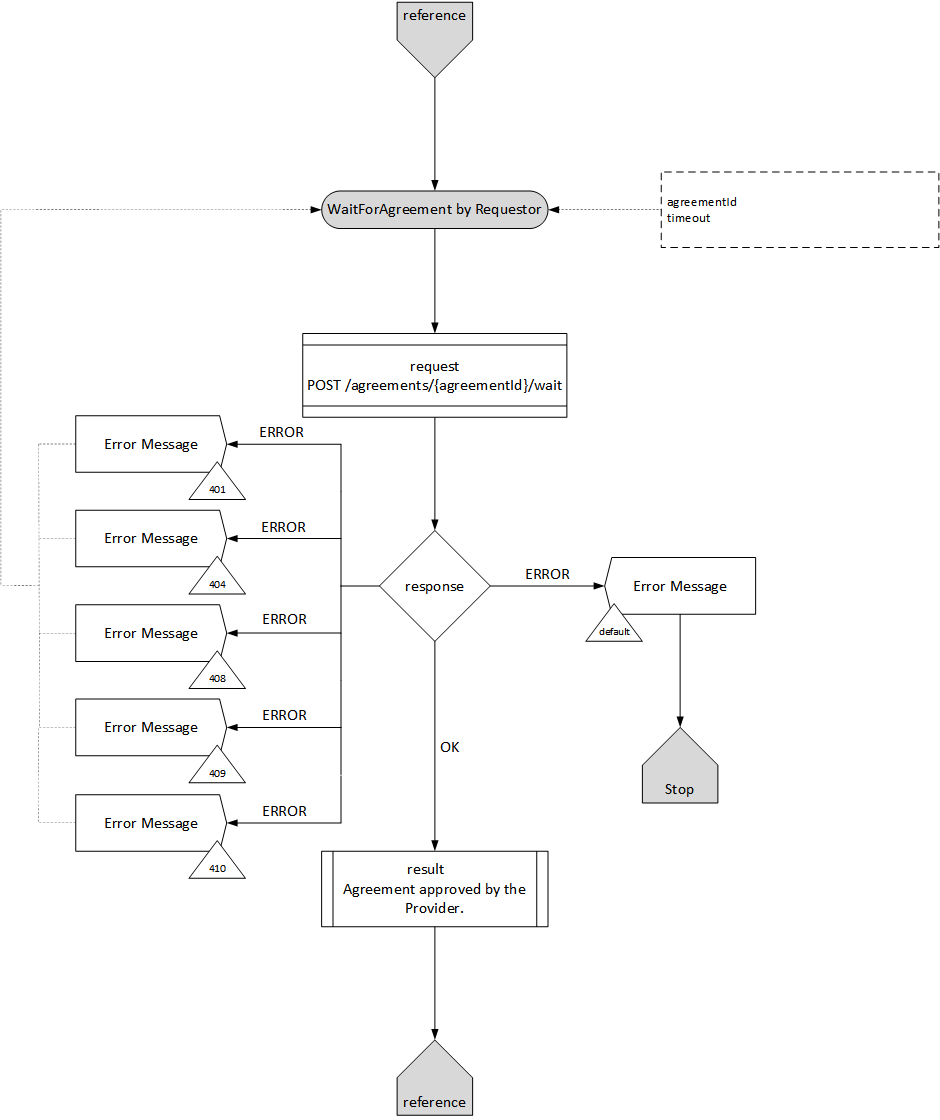
\includegraphics[width=11cm,height=11cm,angle=0]{./diag/Workflow/Market/WaitForAgreement-R-Workflow.png}
    \caption{Requestor Workflow WaitForApproval }
	\label{fig:RWW}
\end{figure}

\end{enumerate}

\newpage

% ApproveAgreement

\subsubsubsection{ApproveAgreement Function}

\begin{enumerate}

\item Profile

\begin{enumerate}

\item Description

The ApproveAgreement function is used to approve Agreement proposed by Requestor. This method is used by the Provider node. 
It uses the POST /agreements/\{agreementId\}/approve method.

\item Side

Provider

\end{enumerate}

\item Request

\begin{enumerate}

\item Input

\begin{tcolorbox}[boxrule=0pt, frame empty]
\begin{verbatim}

agreementId
appSessionId
timeout

\end{verbatim}
\end{tcolorbox}

%Object
%\begin{tcolorbox}[boxrule=0pt, frame empty]
%\begin{verbatim}
%{
%  "message": "string",
%  "additionalProp1": {}
%}
%\end{verbatim}
%\end{tcolorbox}

\begin{table}[H]
\footnotesize

\begin{center}
\begin{tabular}{|p{3cm}|l|p{3cm}|p{3cm}|p{4cm}|} 
\hline
\rowcolor{lightgray}	Name	& MO.	& Type	& Example & 	Description \\
\hline

agreementId		& M & 	string				&		& 	Agreement Identifier \\
\hline

appSessionId	& O	& 	string				&		&	A correlation/session identifier used for querying events related to an action where this appSessionId has been specified 	\\ 
\hline

timeout			& O & 	number(\$float)		&	5 	&  Timeout used in blocking calls waiting for eg. acknowledgement. 
														How many seconds server should wait for response/acknowledgement of an action 
														(0.0 means it should wait for other party's response indefinitely) \\
\hline
\end{tabular}
\end{center}

\end{table}

\item REST Method

\begin{tcolorbox}[boxrule=0pt, frame empty]
\begin{verbatim} 

POST /agreements/{agreementId}/approve

\end{verbatim}
\end{tcolorbox}

\end{enumerate}

\item Response

\begin{table}[H]
\footnotesize

\begin{center}
\begin{tabular}{|c|l|} 
\hline
\rowcolor{lightgray}	Code 		& 	Description \\
\hline
204	 		&	Agreement approved. \\
\hline
404			&	(404) The specified resource was not found. \\
\hline
401			&	(401) Authorization information is missing or invalid. \\
\hline
408			&	(408) Timeout. \\
\hline
410			&	(410) Gone \\
\hline
default		&	Unexpected error. \\
\hline
\end{tabular}
\end{center}

\end{table}

\item Result

\begin{tcolorbox}[boxrule=0pt, frame empty]
\begin{verbatim}

None

\end{verbatim}
\end{tcolorbox}

%\begin{center}
%\begin{tabular}{|p{3cm}|l|p{3cm}|p{3cm}|p{4cm}|} 
%\hline
%\rowcolor{lightgray}	Name	& MO.	& Type	& Example & 	Description \\
%\hline
%agreementId		& 	& 	string				&						&	Agreement Identyfier \\ 
%\hline
%eventDate		& 	& 	string(\$date-time)	&	YYYY-MM-DDThh:mm:ss.sssZ	&	 \\ 
%\hline
%eventType		& 	& 	string(enum)		&	 &	Event Type \\ 
%\hline
%\end{tabular}
%\end{center}

\item Workflow

(Please see Figure ~\ref{fig:PAA} on page ~\pageref{fig:PAA}):

\begin{figure}[H]
    \centering
    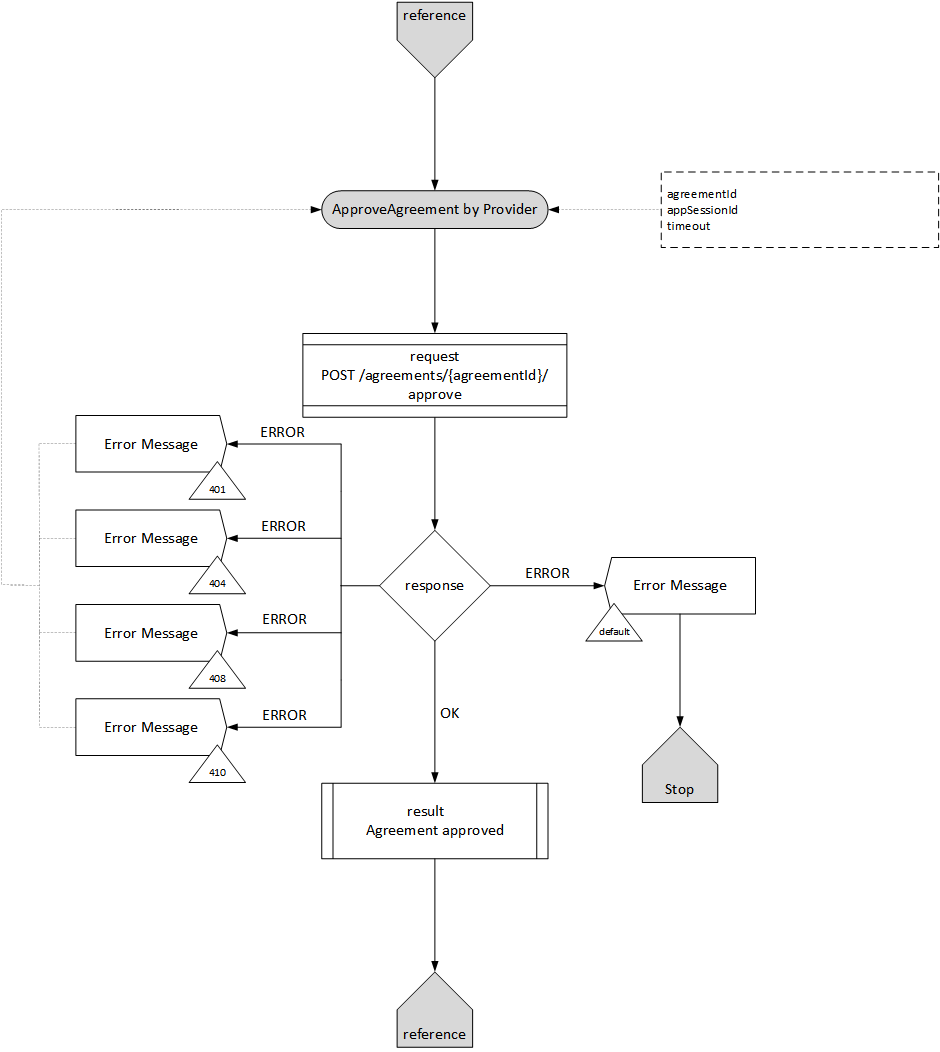
\includegraphics[width=11cm,height=11cm,angle=0]{./diag/Workflow/Market/ApproveAgreement-P-Workflow.png}
    \caption{Provider Workflow Approve Agreement  }
	\label{fig:PAA}
\end{figure}

\end{enumerate}

\newpage

% RejectAgreement

\subsubsubsection{RejectAgreement Function}

\begin{enumerate}

\item Profile

\begin{enumerate}

\item Description

The RejectAgreement function is used to reject Agreement object proposed by Requestor. This method is used by the Provider node. 
It uses the POST /agreements/\{agreementId\}/reject method.

\item Side

Provider

\end{enumerate}

\item Request

\begin{enumerate}

\item Input

\begin{tcolorbox}[boxrule=0pt, frame empty]
\begin{verbatim}

agreementId

\end{verbatim}
\end{tcolorbox}

Object
\begin{tcolorbox}[boxrule=0pt, frame empty]
\begin{verbatim}
{
  "message": "string",
  "additionalProp1": {}
}
\end{verbatim}
\end{tcolorbox}

\begin{table}[H]
\footnotesize

\begin{center}
\begin{tabular}{|p{3cm}|l|p{3cm}|p{3cm}|p{4cm}|} 
\hline
\rowcolor{lightgray}	Name	& MO.	& Type	& Example & 	Description \\
\hline

agreementId		& M & 	string				&		& 	Agreement Identifier \\
\hline

message 		& O	& 	string				&		&	 	\\ 
\hline

additionalProp1 & O	& 	json				&		&	 	\\ 
\hline

\end{tabular}
\end{center}

\end{table}

\item REST Method

\begin{tcolorbox}[boxrule=0pt, frame empty]
\begin{verbatim} 

POST /agreements/{agreementId}/reject

\end{verbatim}
\end{tcolorbox}

\end{enumerate}

\item Response

\begin{table}[H]
\footnotesize

\begin{center}
\begin{tabular}{|c|l|} 
\hline
\rowcolor{lightgray}	Code 		& 	Description \\
\hline
204	 		&	Agreement rejected. \\
\hline
404			&	(404) The specified resource was not found. \\
\hline
401			&	(401) Authorization information is missing or invalid. \\
\hline
410			&	(410) Gone \\
\hline
default		&	Unexpected error. \\
\hline
\end{tabular}
\end{center}

\end{table}

\item Result

\begin{tcolorbox}[boxrule=0pt, frame empty]
\begin{verbatim}

None

\end{verbatim}
\end{tcolorbox}

%\begin{center}
%\begin{tabular}{|p{3cm}|l|p{3cm}|p{3cm}|p{4cm}|} 
%\hline
%\rowcolor{lightgray}	Name	& MO.	& Type	& Example & 	Description \\
%\hline
%agreementId		& 	& 	string				&						&	Agreement Identyfier \\ 
%\hline
%eventDate		& 	& 	string(\$date-time)	&	YYYY-MM-DDThh:mm:ss.sssZ	&	 \\ 
%\hline
%eventType		& 	& 	string(enum)		&	 &	Event Type \\ 
%\hline
%\end{tabular}
%\end{center}

\item Workflow

(Please see Figure ~\ref{fig:PRA} on page ~\pageref{fig:PRA}):

\begin{figure}[H]
    \centering
    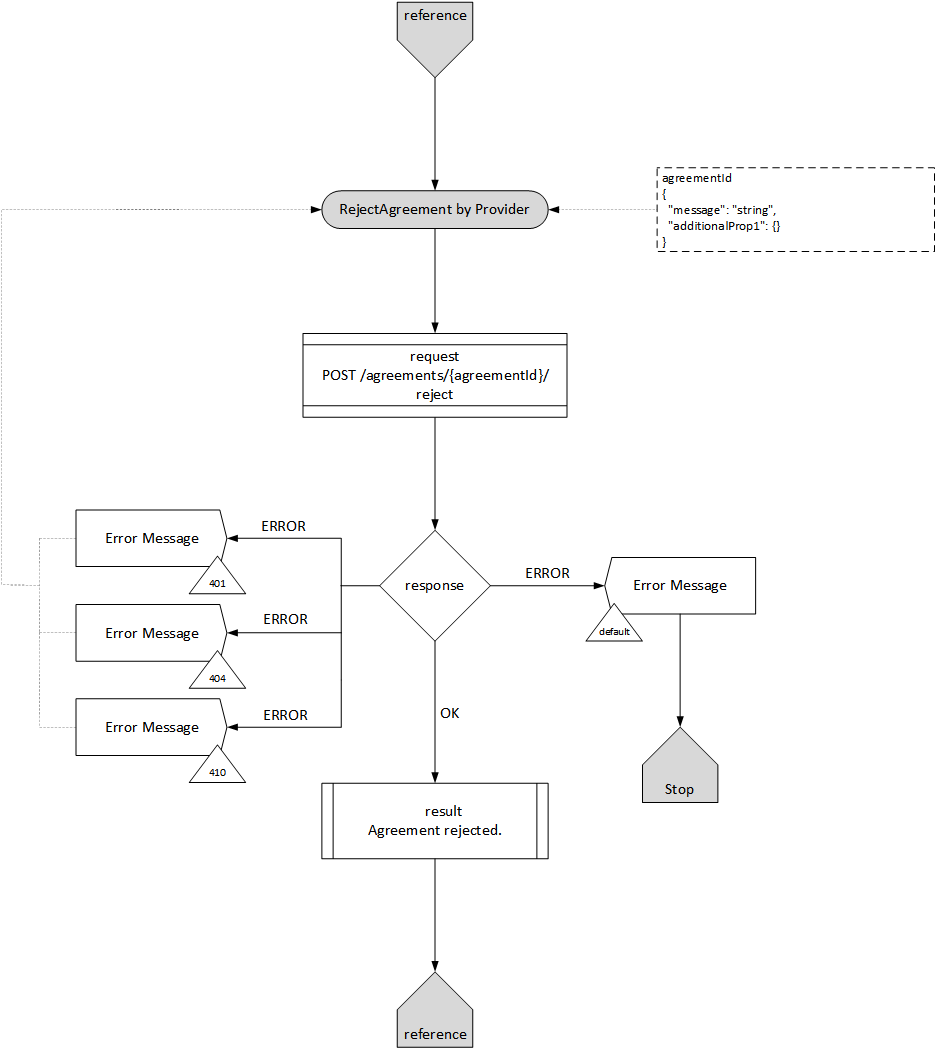
\includegraphics[width=11cm,height=11cm,angle=0]{./diag/Workflow/Market/RejectAgreement-P-Workflow.png}
    \caption{Provider Workflow Reject Agreement  }
	\label{fig:PRA}
\end{figure}

\end{enumerate}

\newpage

